%%%%%%%%%%%%%%%%%%%%%%%%%%%%%%%%%%%%%%%%%%%%%%%%%%%%%%%%%%%%%%%%%%%%%%%%%%
%% Draft submission to INFORMS Journal on Computing (IJOC).
%% Built from the official INFORMS-IJOC-Template (v. Feb 2026).
%%%%%%%%%%%%%%%%%%%%%%%%%%%%%%%%%%%%%%%%%%%%%%%%%%%%%%%%%%%%%%%%%%%%%%%%%%
\documentclass[ijoc,sglanonrev]{informs4}
\usepackage{eqndefns-left}
\RequirePackage{tgtermes}
\RequirePackage{newtxtext}
\RequirePackage{newtxmath}
\RequirePackage{bm}
\RequirePackage{endnotes}

\OneAndAHalfSpacedXII

\usepackage{algorithm}
\usepackage{algpseudocode}
\usepackage{amsfonts}

\usepackage{natbib}
 \bibpunct[, ]{(}{)}{,}{a}{}{,}%
 \def\bibfont{\small}%
 \def\bibsep{\smallskipamount}%
 \def\bibhang{24pt}%
 \def\newblock{\ }%
 \def\BIBand{and}%

\EquationsNumberedThrough
\TheoremsNumberedThrough
\ECRepeatTheorems

\MANUSCRIPTNO{}

% Convenience macros
\newcommand{\Rspread}{R}
\newcommand{\FF}{F}

\begin{document}

\RUNAUTHOR{Dang}

\RUNTITLE{Adaptive Influence Minimization by Deferred Blocking}

\TITLE{Adaptive Influence Minimization via Deferred Frontier Blocking: Theory, Algorithms, and Exact Validation on Bounded-Treewidth Graphs}

\ARTICLEAUTHORS{%
\AUTHOR{Quang-Vinh Dang}
\AFF{British University Vietnam, Hung Yen, Vietnam, \EMAIL{vinh.dq4@buv.edu.vn}}
}

\ABSTRACT{%
\textit{Research Questions.} Blocking the further spread of an
already-seeded rumor or epidemic on a network, by disabling a small number
of accounts or individuals under a fixed budget, is normally solved as a
one-shot decision: the entire budget is spent before anything about how
the outbreak actually unfolds is observed. We ask two questions this
one-shot view leaves open. First, can a decision maker who instead commits
the budget gradually, as the outbreak reveals itself, ever do worse than
committing everything up front, and by how much better can they do?
Second, since every existing method for choosing which accounts to disable
is judged by randomly simulating the outbreak many times rather than by
computing its true effect, how far off can that simulation-based judgment
be from the truth?

\textit{Methodology and Results.} We answer the first question with DEFER,
a general procedure that upgrades any existing one-shot blocking method
into a gradual one, and we prove three things about it: gradual commitment
never leaves the decision maker worse off than committing everything
immediately; a simple rule for deciding when to commit versus wait is the
best possible such rule under natural local conditions; and the advantage
of committing gradually over committing all at once can be made arbitrarily
large, growing with how many people a typical infected individual can pass
the outbreak to. We answer the second question with TWIG, a method that
computes the exact effect of any proposed blocking choice, rather than
estimating it by simulation, on networks small enough for exact computation,
and we use it to measure -- for the first time without simulation noise
clouding the measurement -- how often and how badly the commonly used
greedy blocking heuristic misses the truly best choice.

\textit{Importance and Implications.} Public-health authorities and
platform moderators rarely have to decide everything about an intervention
before it begins; DEFER shows, with a formal guarantee rather than a case
study, that using this flexibility is never harmful and can be highly
valuable, and it does so by wrapping methods practitioners already use
rather than by replacing them. TWIG supplies a rigorous check on the
simulation-based evaluations that the entire outbreak-blocking literature
has relied on until now, exposing a source of error in that literature
that has gone unmeasured.
}%

\FUNDING{The author received no external funding for this research.}

\KEYWORDS{influence minimization, adaptive optimization, misinformation blocking, treewidth, dynamic programming, network science}

\maketitle
%%%%%%%%%%%%%%%%%%%%%%%%%%%%%%%%%%%%%%%%%%%%%%%%%%%%%%%%%%%%%%%%%%%%%%

\section{Introduction}\label{sec:intro}

Misinformation and epidemic-style contagions on networks share a common
downstream control problem once they have already started: given a fixed
set of active or seeded sources and a limited budget of vertices that can be
removed (accounts suspended, individuals quarantined, links cut), which
vertices should be chosen to minimize the eventual spread? This is the
\emph{influence minimization} (IMIN) problem \citep{xie2023,xie2024}, the
natural complement of the much more heavily studied influence
\emph{maximization} problem \citep{kempe2003}: instead of choosing seeds to
spread a cascade, IMIN chooses a small blocking set to contain one. Unlike
maximization, the objective is not supermodular in general, so greedy
selection carries no approximation guarantee, and the problem is NP-hard and
hard to approximate \citep{xie2023}.

Every published IMIN algorithm -- AdvancedGreedy and GreedyReplace
\citep{xie2023,xie2024}, and the Sandwich lower/upper-bound family -- is
\emph{one-shot}: the entire budget is spent before the cascade is observed
even once. In practice a moderator or public-health authority does not have
to decide everything up front. They observe who has already been exposed,
round by round, and can adapt. This raises two questions that, to our
knowledge, have not been formally answered for IMIN: (i) can adapting to the
unfolding cascade only help, never hurt, relative to any one-shot plan; and
(ii) how large can the benefit of adaptivity be, in the worst case? A third,
orthogonal problem is one of verification: every existing IMIN algorithm is
evaluated by Monte-Carlo simulation of the cascade, so a reported
``optimality gap'' of greedy selection is always confounded with sampling
noise, and no exact ground truth has been available at any scale beyond
trivial instances.

\subsection*{Contributions}
\begin{enumerate}
\item \textbf{DEFER} (Section~\ref{sec:defer}), an adaptive wrapper around
  any one-shot IMIN planner. At each round it plans on the currently
  reachable region, protects the previous round's uncommitted plan against
  being replaced by a worse one, and commits a planned vertex only if a
  simple push-down inequality shows that waiting is not preferable. We
  prove: deferred commitment alone is free (Lemma~\ref{lem:defer-free});
  DEFER weakly dominates the one-shot planner it wraps
  (Theorem~\ref{thm:defer-dominates}); the push-down rule is the myopic
  optimum for the local commit-now/wait decision (Lemma~\ref{lem:pushdown});
  and the adaptivity gap of IMIN is unbounded, growing linearly in the
  maximum out-degree as the activation probability shrinks
  (Theorem~\ref{thm:adaptivity-gap}), with a matching, checkable
  construction.
\item \textbf{TWIG} (Section~\ref{sec:twig}), an exact dynamic program for
  the expected spread of a candidate blocking set on graphs of bounded
  treewidth, proved correct (Theorem~\ref{thm:twig-correct}) and then
  reformulated, via an exact linear-aggregation collapse
  (Theorem~\ref{thm:twig-collapse}), into a genuinely fixed-parameter
  tractable algorithm rather than merely an XP one
  (Propositions~\ref{prop:xp-space}--\ref{prop:fpt-space}). We further prove
  that the direction in which an elimination order is processed is not a
  tuning detail but a first-class algorithmic choice
  (Proposition~\ref{prop:direction}), with a worst-case family (the star
  graph) on which the wrong direction forces the frontier to scale with $n$
  even though the treewidth is $1$.
\item An exact, sampling-noise-free measurement of the optimality gap of
  greedy IMIN selection (Section~\ref{sec:twig-empirical}): on graphs small
  enough for TWIG to enumerate, greedy is exactly optimal in 56 of 60
  instances and departs from the true optimum by up to 84.6\% in the worst
  case found -- the first such measurement in the IMIN literature free of
  Monte-Carlo confounds.
\item A benchmark of DEFER against AdvancedGreedy, GreedyReplace, and
  simple heuristics on SNAP-scale contact and collaboration networks
  (Section~\ref{sec:experiments}), together with an auxiliary,
  apples-to-apples comparison on the companion source-detection problem
  used throughout our broader project.
\end{enumerate}

\subsection{Related Work}\label{sec:related}

\textbf{Influence minimization.} \citet{xie2023} introduce IMIN, prove
NP-hardness and inapproximability, and give AdvancedGreedy. \citet{xie2024}
extend this with GreedyReplace and Sandwich-style bounds and give the
network-reliability-flavored complexity analysis that our Theorem
\ref{thm:twig-correct} builds on for exact verification; their own
Exact-vs-GreedyReplace check (their Table 3) uses a borrowed exact method on
100-node subgraphs at up to four budget levels, considerably smaller and
less systematic than the fully proof-verified, 60-instance study we report
in Section~\ref{sec:twig-empirical}.

\textbf{Rumor and misinformation blocking before IMIN.} The idea of limiting
the damage of an already-spreading process by removing or countering a
small set of vertices predates IMIN's formal NP-hardness treatment by over
a decade. \citet{budak2011} counter-seed a rival campaign under the
independent-cascade model; \citet{he2012} extend this to a competitive
linear-threshold setting; \citet{nguyen2012} and \citet{wang2013blocking}
study node/edge removal directly, essentially the one-shot IMIN objective,
without the hardness or approximation-inapproximability results
\citet{xie2023} later supply; \citet{fan2013} add an explicit removal-cost
budget; \citet{wang2016drimux} and \citet{tong2018} generalize to dynamic
and multi-campaign rumor environments; \citet{tong2017} give a
$(1-1/e-\delta)$-style guarantee via reverse-reachable sampling for a
closely related blocking-maximization objective; \citet{farajtabar2017}
instead model the cascade as a Hawkes process and steer it with
reinforcement learning rather than one-time vertex removal; \citet{yan2020}
study blocker placement under a fixed removal budget; \citeauthor{zareie2021}
survey this pre-2021 line. \citet{xiang2024} and \citet{xie2024pvldb} are
recent variants (a pertinence-constrained version, and a dual
vertex-countering formulation) contemporaneous with \citet{xie2024}, the
direct ancestor of the AG/GR planners DEFER wraps. None of this line
considers the timing of commitment as a decision variable in its own
right, which is the gap DEFER's adaptive formulation addresses.

\textbf{Exact spread computation.} Computing expected spread exactly is a
network-reliability problem and is \#P-hard in general
\citep{valiant1979,provan1983}. \citet{nakamura2026} give a linear-time
exact algorithm for expected influence spread on bounded-\emph{pathwidth}
graphs; their result computes spread only and does not address blocking set
selection, greedy verification, or the adaptive setting, and pathwidth is a
strictly more restrictive parameter than the treewidth TWIG uses. Our
treewidth dynamic program follows the classical bounded-treewidth
programming paradigm \citep{bodlaender1988,cygan2015}.

\textbf{Adaptive submodular and sequential decision problems.} Adaptive
variants of influence \emph{maximization} and related coverage problems are
well studied; to our knowledge no prior work formalizes an adaptive variant
of IMIN or proves a lemma of the shape of Lemma~\ref{lem:defer-free} (that
deferred commitment of a fixed one-shot plan is loss-free) or an
unbounded-adaptivity-gap result of the shape of
Theorem~\ref{thm:adaptivity-gap} for this problem.

\section{Preliminaries}\label{sec:prelim}

\subsection{The independent cascade model}\label{sec:ic-model}

$G=(V,E)$ is a directed graph,
$n=|V|$, $m=|E|$, with edge probabilities $p:E\to(0,1]$. A live-edge
realization $\omega\in\{0,1\}^E$ is drawn with
$\Pr[\omega]=\prod_{e}p_e^{\omega_e}(1-p_e)^{1-\omega_e}$. For a seed set
$S\subseteq V$ and blocked set $B\subseteq V\setminus S$, write
$G_B=G[V\setminus B]$ and let $\Rspread(\omega,B)\subseteq V\setminus B$ be
the set of vertices reachable from $S$ using only live edges of $G_B$. The
\emph{expected spread} is
\begin{equation}\label{eq:spread}
\FF(B)\;=\;\mathbb E_\omega\bigl[\,|\Rspread(\omega,B)\setminus S|\,\bigr].
\end{equation}

\subsection{Problem formalization}\label{sec:formalization}

\begin{definition}[IMIN, one-shot]\label{def:imin}
Given $G$, $p$, seed set $S$, and budget $b\in\mathbb N$, the
\emph{influence minimization} (IMIN) problem is
\begin{equation}\label{eq:imin}
\min_{B\subseteq V\setminus S}\ \FF(B)
\qquad\text{subject to}\qquad
|B|\le b.
\end{equation}
\end{definition}

\noindent \citet{xie2023} show Problem~\eqref{eq:imin} is NP-hard and hard
to approximate within any constant factor unless P$=$NP, and that $\FF$ is
not supermodular in $B$ under the IC model, so the greedy
$(1-1/e)$-guarantee available for influence \emph{maximization}
\citep{kempe2003} does not transfer.

To formalize the adaptive variant, let a \emph{history} up to round $t$ be
$h_t=(N_0,N_1,\dots,N_t)$, the sequence of newly activated sets observed so
far (full-adoption feedback: which vertices activate each round, not which
live edges carried the activation). Let $\mathcal H$ denote the set of all
histories of any length.

\begin{definition}[Adaptive policy]\label{def:policy}
An \emph{adaptive blocking policy} is a function
$\pi:\mathcal H\to 2^V$ mapping each history $h_t$ to a set of
not-yet-activated, not-yet-blocked vertices to additionally block in round
$t+1$, subject to $\sum_{t}|\pi(h_t)|\le b$ over the run of the cascade.
Write $\sigma(\pi)$ for the (random) final spread beyond $S$ that results
from running the cascade under policy $\pi$.
\end{definition}

\begin{definition}[IMIN, adaptive]\label{def:adaptive-imin}
Given $G$, $p$, $S$, and budget $b$, the \emph{adaptive} IMIN problem is
\begin{equation}\label{eq:adaptive-imin}
\min_{\pi}\ \mathbb E\bigl[\sigma(\pi)\bigr]
\qquad\text{subject to}\qquad
\textstyle\sum_t|\pi(h_t)|\le b\ \text{a.s.}
\end{equation}
A one-shot policy is the special case $\pi(h_0)=B$ for a fixed
$B$ with $|B|\le b$ and $\pi(h_t)=\varnothing$ for $t\ge1$, so
Problem~\eqref{eq:imin} is exactly Problem~\eqref{eq:adaptive-imin}
restricted to one-shot policies, and
$\min_\pi\mathbb E[\sigma(\pi)]\le\min_{|B|\le b}\FF(B)$ trivially, since
every one-shot policy is a feasible (adaptive) policy. The
\emph{adaptivity gap} of an instance is the ratio of the right-hand side to
the left-hand side of this inequality; Theorem~\ref{thm:adaptivity-gap}
shows this gap is unbounded.
\end{definition}

DEFER (Section~\ref{sec:defer}) is a construction of a specific policy
$\pi_{\mathrm{DEFER}}$, parameterized by a choice of one-shot planner
$\mathcal P$, that is feasible for Problem~\eqref{eq:adaptive-imin} and
provably close to optimal relative to $\mathcal P$'s own one-shot value
(Theorem~\ref{thm:defer-dominates}). TWIG (Section~\ref{sec:twig}) instead
addresses an orthogonal computational issue in Problem~\eqref{eq:imin}
itself: $\FF(B)$, the objective being optimized, is a \#P-hard quantity to
evaluate exactly \citep{valiant1979,provan1983}, so every algorithm for
either problem above that a practitioner actually runs replaces $\FF(B)$
with a Monte-Carlo estimate; TWIG computes $\FF(B)$ exactly instead, on
graphs where doing so is tractable, to certify how much error that
replacement introduces.

\subsection{Treewidth machinery}\label{sec:treewidth-prelim}

Used only in Section~\ref{sec:twig}. Fix a
permutation $\sigma=(\sigma_1,\dots,\sigma_n)$ of $V$ and write
$\mathrm{pos}(v)$ for $v$'s index. For $v=\sigma_i$, let
$\mathrm{connect\_to}(v)=\{u\in N(v):\mathrm{pos}(u)<i\}$ and
$\mathrm{last}(v)=\max_{x\in N[v]}\mathrm{pos}(x)$. The \emph{frontier}
after step $i$ is $F_i=\{\sigma_j:j\le i,\ \mathrm{last}(\sigma_j)\ge i\}$,
and the \emph{width} of $\sigma$ is $w=\max_i|F_i|-1$, which upper-bounds
the treewidth of $G$ when $\sigma$ comes from a min-fill-in / min-degree
chordal completion \citep{bodlaender1988,cygan2015}.

Table~\ref{tab:notation} collects the notation introduced above and in
Sections~\ref{sec:defer} and \ref{sec:twig} for reference.

\begin{table}[h]
\TABLE
{Notation used throughout the paper\label{tab:notation}}
{\begin{tabular}{@{}ll@{}}
\hline
\up Symbol & Meaning \\
\hline
\up $G=(V,E)$, $n$, $m$ & graph, vertex count, edge count \\
$p:E\to(0,1]$ & independent-cascade edge probabilities \\
$S$, $B$, $b$ & seed set, blocked set, blocking budget \\
$\omega$, $\Rspread(\omega,B)$ & live-edge realization, reachable set under $\omega$ with $B$ removed \\
$\FF(B)$ & expected spread with blocking set $B$ (Eq.~\ref{eq:spread}) \\
$F_t$, $A_t$, $N_t$ & round-$t$ frontier, active set, newly activated set (DEFER) \\
$P_t$, $L$, $C_t$ & round-$t$ plan, uncommitted leftover, vertices committed this round \\
$q_v$, $c_v$, $\lambda_t$ & exposure probability, child count, shadow price of a budget unit \\
$\mathcal P$ & one-shot planner wrapped by DEFER \\
$\sigma$, $\mathrm{pos}$, $\mathrm{last}$ & elimination order, position function, retirement step (TWIG) \\
$F_i$, $w$ & frontier after step $i$, width of $\sigma$ (TWIG) \\
$\kappa=(\Pi,\rho)$ & configuration: partition plus pending counts (Definition~\ref{def:config}) \\
$P_\kappa$, $\mathrm{acc}$ & configuration probability, running accumulated spread \\
$P_s$, $W_b$ & shape-aggregated probability and weighted pending sum (Theorem~\ref{thm:twig-collapse}) \\
\down $B_{w+1}$ & $(w+1)$-th Bell number \\
\hline
\end{tabular}}
{}
\end{table}

\section{DEFER: Adaptive Influence Minimization by Deferred Frontier Blocking}\label{sec:defer}

\subsection{Algorithm}\label{sec:defer-algo}

DEFER wraps a one-shot planner $\mathcal P$ (any IMIN algorithm; by default
a dominator-tree greedy planner with isolation moves). At each round it
re-plans on the currently reachable region, keeps whichever of the new plan
and the previous round's uncommitted leftover looks better on freshly drawn
samples (\emph{plan protection}), and commits only the fraction of the plan
that is both exposed to the current frontier and passes a push-down test.

\begin{algorithm}[h]
\caption{DEFER}\label{alg:defer}
\begin{algorithmic}[1]
\Require graph $G$, probabilities $p$, seeds $S$, budget $b$, sample size
  $\theta$, one-shot planner $\mathcal P$
\State $A_0\gets S$, $B_0\gets\varnothing$, $F_0\gets S$, $L\gets\varnothing$ (uncommitted leftover)
\For{$t=0,1,2,\dots$ while the cascade is alive and $|B_t|<b$}
  \State $b_t\gets b-|B_t|$
  \State draw $\theta$ live-edge subgraphs reachable from $F_t$ avoiding $A_t\cup B_t$
  \State $P'\gets\mathcal P(\text{seeds}=F_t,\ \text{forbidden}=A_t\cup B_t,\ \text{budget}=b_t)$ on the samples
  \State $P_t\gets\arg\max\{\text{sample-average saving of } P', L\}$ \Comment{plan protection}
  \State $X_t\gets$ inactive, unblocked out-neighbors of $F_t$
  \For{$v\in P_t\cap X_t$}
    \State $q_v\gets 1-\prod_{u\in F_t}(1-p(u,v))$; $c_v\gets$ inactive unblocked out-degree of $v$
    \State $\lambda_t\gets$ smallest marginal saving among the picks of $P_t$ (0 if $P_t$ does not exhaust $b_t$)
    \If{$q_v\,(c_v+1/\lambda_t)\ge 1$} \Comment{push-down rule, Lemma~\ref{lem:pushdown}}
      \State block $v$ now
    \EndIf
  \EndFor
  \State $L\gets P_t\setminus(\text{blocked this round})$
  \State observe $N_{t+1}$; update $A_{t+1},F_{t+1}$
\EndFor
\end{algorithmic}
\end{algorithm}

The push-down rule compares spending one budget unit on an exposed node $v$
now against waiting one round and, if $v$ activates (probability $q_v$),
protecting its $c_v$ children instead while losing $v$ itself. When the
planner is deterministic given the samples and no new information arrives,
DEFER reduces to lazily committing the one-shot planner's own plan
(Lemma~\ref{lem:defer-free}); the two ablations used in
Section~\ref{sec:experiments} are COMMIT (same loop, but the whole plan is
committed every round) and the one-shot planners run without any wrapper.

\subsection{Worked example}\label{sec:defer-example}

We make the mechanism behind Theorem~\ref{thm:adaptivity-gap} concrete on
the star-of-paths instance its proof constructs, with $\Delta=4$ branches,
per-branch activation probability $p=0.1$, path length $L=50$, and budget
$b=1$. Seed $s$ has four out-neighbors $a_1,\dots,a_4$, each independently
live with probability $p$; each $a_i$ that activates starts a private,
deterministic path of $L=50$ further vertices. With no intervention, each
branch contributes $L+1=51$ vertices to the spread with probability $p$,
so the expected total spread is $\Delta p(L+1)=4(0.1)(51)=20.4$.

A one-shot policy with budget 1 must pick a single vertex to remove before
observing anything; by symmetry the best it can do is remove one branch's
gateway $a_i$ outright, which pre-empts that branch's entire contribution
regardless of whether $(s,a_i)$ would have been live. Its expected spread
is then the sum over the remaining three branches,
$(\Delta-1)p(L+1)=3(0.1)(51)=15.3$.

DEFER instead waits one round. It observes $N_1=\{a_i:(s,a_i)\text{ live}\}$
-- the number of active branches $k$ is $\mathrm{Binomial}(4,0.1)$, so
$k=0$ with probability $0.656$, $k=1$ with probability $0.292$, $k=2$ with
probability $0.049$, and $k\ge3$ with probability $0.004$ -- and spends its
one block on the first path vertex of one active branch (blocking $a_i$
itself is no longer possible once it has activated). This seals that one
branch's continuation at a cost of only the vertex $a_i$ already reached,
while $k-1$ other active branches, if any, still propagate their full
length-$L$ path. DEFER's expected spread is
$\Delta p+L\cdot\mathbb E[(k-1)^+]=0.4+50(0.056)=3.205$, using
$\mathbb E[(k-1)^+]=\sum_{k\ge1}(k-1)\Pr[k]=0.056$ computed from the
binomial probabilities above. The realized ratio of one-shot to DEFER
expected spread on this instance is $15.3/3.205\approx4.77$, comfortably
above the headline asymptotic bound of
$(1-(1-p)^\Delta)/p=(1-0.9^4)/0.1\approx3.44$ that
Theorem~\ref{thm:adaptivity-gap} guarantees in the limit; the gap between
the exact ratio and the stated bound is the ``up to an additive constant''
slack in the theorem's proof, which drops lower-order-in-$L$ terms to keep
the bound's statement independent of $L$.

The qualitative point survives far more general instances than this
symmetric construction: a one-shot policy pays for protection whether or
not the threat it is protecting against ever materializes, while DEFER
pays only for the branches that are actually observed to be live. The
push-down rule (Lemma~\ref{lem:pushdown}) is what tells DEFER \emph{when}
this is worth doing -- here, with $c_v=1$ child per branch vertex and
$q_v=p=0.1$ small relative to the branch's shadow price
$\lambda\approx pL/1\approx5$, the condition $q_v(c_v+1/\lambda)<1$ holds
comfortably, so every exposed branch vertex is deferred rather than
committed immediately; on a graph where $q_v$ is close to 1 (a near-certain
threat) the same rule would instead commit right away, recovering one-shot
behavior exactly where deferring would not help.

\subsection{Theoretical guarantees}\label{sec:defer-theory}

Full proofs of every result in this section are given in
Online Supplement~\ref{ec:defer-proofs}.

\begin{lemma}[Deferral is free]\label{lem:defer-free}
Fix a live-edge realization, the seeds, and any set $P$ with $|P|\le b$. Let
$\pi_P$ be the policy that, in every round, blocks the not-yet-blocked
vertices of $P$ that are exposed to the current frontier. Then $\pi_P$
produces exactly the same final active set as blocking $P$ at time $0$, and
blocks at most as many vertices.
\end{lemma}

\begin{theorem}[DEFER weakly dominates its planner]\label{thm:defer-dominates}
Let $P_0$ be $\mathcal P$'s plan at round $0$. If, in every later round, the
planner returns a plan whose sample-average saving is at least that of the
leftover $P_{t-1}\setminus C_{t-1}$ -- guaranteed when the leftover is
offered to the planner as a candidate solution -- then the expected final
spread of DEFER is at most that of the one-shot solution $P_0$, up to the
sampling error of the $\theta$ samples.
\end{theorem}

\begin{lemma}[Push-down is the myopic optimum]\label{lem:pushdown}
Consider an exposed planned vertex $v$ whose children (inactive
out-neighbors) jointly protect the same set as $v$ minus $v$ itself, assume
the children are exposed only through $v$, and value a budget unit at
$\lambda$ vertices. Among the two policies ``block $v$ now'' and ``block
$v$'s children if and only if $v$ activates,'' the second has smaller
expected loss (vertices lost plus $\lambda$ times budget spent) if and only
if $q_v(c_v+1/\lambda)<1$.
\end{lemma}

\begin{theorem}[The adaptivity gap of IMIN is unbounded]\label{thm:adaptivity-gap}
For every $\Delta\ge 2$ and $p\in(0,1)$ there is an instance with maximum
out-degree $\Delta$ on which the best one-shot solution with budget $1$ has
expected spread at least $\bigl(1-(1-p)^{\Delta}\bigr)/p$ times that of DEFER
with budget $1$ (up to an additive constant); this ratio tends to $\Delta$ as
$p\to 0$.
\end{theorem}

\begin{theorem}[Complexity of DEFER]\label{thm:defer-complexity}
Let $n_t,m_t$ be the number of vertices and edges reachable from $F_t$ in
the union of the $\theta$ samples, $r$ the number of rounds, and $\alpha$
the inverse Ackermann function. With the dominator planner, round $t$ costs
$O(\theta\,m_t\,\alpha(m_t,n_t))$ for the dominator trees plus
$O(b_t\,\theta'\,m_t\,\alpha)$ for the greedy picks ($\theta'\le\theta$);
the total is $O\bigl(\sum_t(1+b_t)\,\theta\,m_t\,\alpha\bigr)$, which is
$O(r\,b\,\theta\,m\,\alpha(m,n))$ in the worst case.
\end{theorem}

We additionally construct \texttt{isocut}, a one-shot planner of our own
that adds one further kind of candidate move to AG's planner --
isolating a whole seed's out-neighborhood at once, rather than blocking
one vertex at a time -- and prove it admits a worst-case separation
(Theorem~\ref{thm:isocut-separation}, Online Supplement) from published
one-shot planners: AdvancedGreedy, GreedyReplace, and the Sandwich lower
bound. \texttt{isocut} is not itself a competing baseline from the
literature; it is reported only as an ablation, in
Section~\ref{sec:isocut-practice}, because it is rarely selected on the
SNAP graphs used there.

\begin{theorem}[Isolation-move separation]\label{thm:isocut-separation}
There is a family of instances on which AdvancedGreedy, GreedyReplace, and
the Sandwich lower-bound greedy all save $O(b)$ vertices with budget $b$,
while a planner with frontier-isolation moves saves $\Omega(N)$ for
arbitrary $N$.
\end{theorem}

\section{TWIG: Exact Treewidth-Bounded Validation}\label{sec:twig}

Every quantity reported by a one-shot IMIN heuristic -- including the plans
DEFER wraps -- is normally a Monte-Carlo estimate of Equation
\eqref{eq:spread}, because computing $\FF(B)$ exactly is a network-reliability
computation and is \#P-hard in general \citep{valiant1979,provan1983}. TWIG
computes $\FF(B)$ \emph{exactly} on graphs of bounded treewidth, giving a
ground-truth oracle that we use to certify how close greedy selection comes
to the true optimum, free of sampling noise.

\subsection{Algorithm}\label{sec:twig-algo}

\begin{definition}[Configuration]\label{def:config}
A configuration over a vertex set $F\subseteq V$ is a pair
$\kappa=(\Pi,\rho)$ where $\Pi$ is a set partition of $F$ with at most one
distinguished block $\mathrm{SEED}$, and $\rho$ maps each non-$\mathrm{SEED}$
block to a nonnegative integer (its \emph{pending count}).
\end{definition}

\texttt{ExactSpread} maintains, after each step $i$ of the schedule defined
in Section~\ref{sec:prelim}, a probability distribution over configurations
on the frontier $F_i$, plus a running scalar $\mathrm{acc}_i$, updated by
three operations: \emph{introduce} a new singleton block for each newly
processed vertex; \emph{process\_edge} branches on each edge's live/dead
outcome, merging blocks on the live branch and paying out to $\mathrm{acc}$
when a merge is into $\mathrm{SEED}$; and \emph{retire} pays out $\mathrm{acc}$
for a retiring $\mathrm{SEED}$-block vertex (unless it is itself a seed), or
defers a retiring ordinary vertex into its block's pending count, discarding
that count once the block empties of active members.

\subsection{Worked example}\label{sec:twig-example}

We trace \texttt{ExactSpread} on the smallest instance that already
exercises every case of Definition~\ref{def:config}: the path
$1$--$2$--$3$--$4$, seed $S=\{1\}$, no blocking ($B=\varnothing$), and edge
probabilities $p_{12}=p_{23}=p_{34}=0.5$. The elimination order is the
natural order $1,2,3,4$ (a path has treewidth 1 and either direction keeps
the frontier at size $\le2$). Directly, $F(\varnothing)=\Pr[2\text{
reached}]+\Pr[3\text{ reached}]+\Pr[4\text{ reached}]
=p_{12}+p_{12}p_{23}+p_{12}p_{23}p_{34}=0.5+0.25+0.125=0.875$.

\texttt{ExactSpread} reaches the same number without ever conditioning on
all $2^3=8$ live-edge histories explicitly. After introducing vertex 1
(the seed, a singleton SEED block) and vertex 2, \emph{process\_edge}(1,2)
branches: with probability $0.5$ nothing changes; with probability $0.5$
vertex 2 merges into SEED (with pending $0$, so this merge pays out $0$
into $\mathrm{acc}$, since no previously-retired vertex was waiting on this
block). Vertex 1 then retires; being a seed, it is excluded from the
payout by Definition~\ref{def:config}'s retire rule, so $\mathrm{acc}$ is
still $0$ after step 1, and the frontier now holds two configurations:
$\{2\}$ ordinary with probability $0.5$, or $\{2\}\equiv\mathrm{SEED}$ with
probability $0.5$. The same branching repeats at vertex 3 (splitting each
of the two configurations in two, by whether $(2,3)$ is live) and at vertex
4. Vertex 2 retires at step 2: in the two configurations where its block is
SEED (combined probability $0.5$, from $(1,2)$ live), Definition
\ref{def:config}'s payout rule contributes $\mathrm{acc}\mathrel{+}=0.5$
(vertex 2 is reached with probability exactly $p_{12}$); in the other two,
its ordinary block either merges into a later live edge (deferring its
now-nonexistent pending count, moot here since $\rho=0$) or is discarded
with no payout, correctly reflecting that a component disconnected from
the seed is never reached. Table~\ref{tab:twig-example} lists all eight
live-edge histories, grouped by the configuration \texttt{ExactSpread}
places them in; summing $P_\kappa$ over the histories where each vertex's
block is SEED at its retirement reproduces
$\Pr[2\text{ reached}]=0.5$, $\Pr[3\text{ reached}]=0.25$,
$\Pr[4\text{ reached}]=0.125$, and the running total after vertex 4's
retirement is exactly $0.5+0.25+0.125=0.875=F(\varnothing)$, matching the
closed form and Theorem~\ref{thm:twig-correct}.

\begin{table}[h]
\TABLE
{The eight live-edge histories of the path example, grouped by outcome\label{tab:twig-example}}
{\begin{tabular}{@{}ccccc@{}}
\hline
\up $(1,2)$ & $(2,3)$ & $(3,4)$ & $\Pr$ & reached ($\subseteq\{2,3,4\}$) \\
\hline
\up dead & dead & dead & 0.125 & $\varnothing$ \\
dead & dead & live & 0.125 & $\varnothing$ \\
dead & live & dead & 0.125 & $\varnothing$ \\
dead & live & live & 0.125 & $\varnothing$ \\
live & dead & dead & 0.125 & $\{2\}$ \\
live & dead & live & 0.125 & $\{2\}$ \\
live & live & dead & 0.125 & $\{2,3\}$ \\
\down live & live & live & 0.125 & $\{2,3,4\}$ \\
\hline
\end{tabular}}
{Four histories (rows 2, 4, 6, 8, and 7 for vertex 4 only) show that the
identity of which \emph{other} downstream edges are live does not affect
whether an already-connected vertex is reached, which is exactly the
redundancy \texttt{ExactSpread} exploits by merging histories into shared
configurations rather than enumerating them.}
\end{table}

\begin{theorem}[Correctness of \texttt{ExactSpread}]\label{thm:twig-correct}
For every $B$, \texttt{ExactSpread}$(G,p,S)$.evaluate$(B)=\FF(B)$.
\end{theorem}

\subsection{Complexity: from XP to FPT in treewidth}\label{sec:twig-complexity}

\begin{proposition}[State space of \texttt{ExactSpread}]\label{prop:xp-space}
The number of distinct configurations at any step is at most
$B_{w+1}\cdot(n+1)^{w+1}$, where $B_{w+1}$ is the $(w+1)$-th Bell number.
\end{proposition}

This makes \texttt{ExactSpread} XP, not FPT, in treewidth: the degree of the
polynomial in $n$ grows with $w$.

\begin{theorem}[Correctness of the linear-aggregation collapse]\label{thm:twig-collapse}
Fix a partition shape $s$ and, at some step, let
$\mathcal K_s=\{(s,\rho):P_{(s,\rho)}>0\}$. Define the aggregates
$P_s=\sum_{(s,\rho)\in\mathcal K_s}P_{(s,\rho)}$ and
$W_b=\sum_{(s,\rho)\in\mathcal K_s}P_{(s,\rho)}\cdot\rho(b)$ for each
non-$\mathrm{SEED}$ block $b$ of $s$. Then $(P_s,\{W_b\})_s$ can be updated
at every step by the four rules \texttt{ExactSpreadFast} implements, and
this update yields the identical sequence of $\mathrm{acc}$ increments as
\texttt{ExactSpread}, for every $B$.
\end{theorem}

\begin{proposition}[State space of \texttt{ExactSpreadFast}]\label{prop:fpt-space}
The number of distinct states at any step is at most $B_{w+1}$, independent
of $n$, giving overall running time $O(n\cdot B_{w+1}\cdot\mathrm{poly}(w))$.
\end{proposition}

Proposition~\ref{prop:fpt-space} is a genuine change of complexity class
from Proposition~\ref{prop:xp-space}, not merely a constant-factor speed-up:
the $n^{w+1}$ factor is eliminated entirely.

\subsection{Processing direction is a first-class algorithmic choice}\label{sec:twig-direction}

\begin{proposition}[Star graphs separate forward and reversed elimination order]\label{prop:direction}
Let $T_k$ be the star $K_{1,k}$, $n=k+1$. Min-fill-in computes the
elimination order $\pi=(\ell_1,\dots,\ell_k,c)$, correctly certifying
treewidth $1$. Running the schedule of Section~\ref{sec:prelim} directly on
$\pi$ (the centre processed last) produces a frontier of size $k=n-1$
immediately before the centre's step. Running it on $\mathrm{reverse}(\pi)$
(the centre processed first) keeps the frontier at size at most $2$
throughout.
\end{proposition}

This is a worst-case separation on an exact, checkable family: a
bounded-treewidth graph (here, treewidth $1$, for any $n$) on which the
\emph{same} elimination order, run in the wrong direction, forces the true
state space of the dynamic program to scale with $n$ instead of remaining
bounded by a function of the width alone. In our implementation the
elimination order is therefore always reversed before scheduling.

\subsection{Empirical validation}\label{sec:twig-empirical}

Combining the collapse of Theorem~\ref{thm:twig-collapse} with the reversed
processing order of Proposition~\ref{prop:direction} makes exact evaluation
tractable on real, non-synthetic small networks:

\begin{table}[h]
\TABLE
{Exact evaluation feasibility on real small networks\label{tab:twig-feasibility}}
{\begin{tabular}{@{}lccc@{}}
\hline
\up Network & $n$ & width (min-fill-in) & \texttt{ExactSpreadFast.evaluate()} \\
\hline
\up Zachary karate club & 34 & 5 & 2.5 s \\
Iceland (sexual contact) & 75 & 4 & 51 s \\
\down Dolphin social network & 62 & $\sim$10--11 & infeasible (memory) \\
\hline
\end{tabular}}
{Before both fixes (Theorem~\ref{thm:twig-collapse} and reversed processing order), karate did not finish in 60 s and Iceland/Dolphin were not attempted.}
\end{table}

On the karate club network (one seed, random independent-cascade
probabilities in $[0.05,0.4]$), \texttt{greedy\_exact} -- greedy selection
using \texttt{ExactSpreadFast} itself as the marginal-gain oracle, with zero
sampling noise -- selects node 2 at budget 1 (expected spread falls from the
unblocked value to 7.98) and adds node 1 at budget 2 (expected spread
5.51). \citet{xie2023} prove $\FF(\cdot)$ is not supermodular in $B$ under
the independent-cascade model, so greedy carries no $(1-1/e)$-style
guarantee for IMIN, and \citet{xie2024} further show IMIN is APX-hard;
consistent with both results, comparing \texttt{greedy\_exact} against
\texttt{brute\_force\_optimal\_block} on 60 small random instances
($n=6$--$14$, budget 1--4) finds greedy exactly optimal in 56 of 60 and
strictly suboptimal in 4, by up to 84.6\% relative excess spread in the
worst case (mean excess 2.2\% across all 60). This is, to our knowledge, the
first exact (not Monte-Carlo-confounded) measurement of how often and how
badly greedy departs from optimal IMIN selection.

\subsection{Complexity comparison}\label{sec:complexity-comparison}

Table~\ref{tab:complexity} collects the time complexity of every method
this paper compares against or introduces, so the cost of DEFER's
adaptivity and of TWIG's exactness can be read off against the published
one-shot planners in one place. Three points are worth stating explicitly.
First, DEFER's cost (Theorem~\ref{thm:defer-complexity}) is exactly AG's
per-round cost multiplied by the number of rounds $r$: adaptivity is not
free computationally, even though Theorem~\ref{thm:defer-dominates} shows
it is free in expected-spread terms. Second, TWIG's two variants solve a
strictly harder problem than AG/GR/DEFER (exact evaluation of $\FF(B)$
rather than an unbiased Monte-Carlo estimate of it) and are not drop-in
replacements for the sampling-based planners at the graph sizes those
planners target; Proposition~\ref{prop:fpt-space}'s
$n$-independence is what makes \texttt{ExactSpreadFast} usable at all
compared to the brute-force alternative of enumerating all $2^m$ live-edge
realizations, but $B_{w+1}$ still grows very quickly in the treewidth $w$
(Table~\ref{tab:bell-numbers}). Third, \texttt{brute\_force\_optimal\_block}
compounds TWIG's per-evaluation cost with an outer search over all
size-$\le b$ subsets, which is what confines
Section~\ref{sec:twig-empirical}'s optimality-gap study to $n\le14$.

\begin{table}[h]
\TABLE
{Time complexity of every method compared in this paper\label{tab:complexity}}
{\begin{tabular}{@{}ll@{}}
\hline
\up Method & Time complexity \\
\hline
\up AG \citep{xie2024} & $O(b\,\theta\,m\,\alpha(m,n))$ \\
GR \citep{xie2024} & $O(\min\{d^{out}_S,b\}\,\theta\,m\,\alpha(m,n))$ plus a replacement pass \\
DEFER (Theorem~\ref{thm:defer-complexity}) & $O(r\,b\,\theta\,m\,\alpha(m,n))$ ($r$ = number of rounds) \\
\texttt{ExactSpread} (Proposition~\ref{prop:xp-space}) & one \texttt{evaluate}: $O(n\cdot B_{w+1}\cdot(n+1)^{w+1})$ (XP in $w$) \\
\texttt{ExactSpreadFast} (Proposition~\ref{prop:fpt-space}) & one \texttt{evaluate}: $O(n\cdot B_{w+1}\cdot\mathrm{poly}(w))$ (FPT in $w$) \\
\texttt{greedy\_exact} & $O(b)$ \texttt{evaluate} calls, each as above \\
\down \texttt{brute\_force\_optimal\_block} & $O(n^b)$ \texttt{evaluate} calls, each as above \\
\hline
\end{tabular}}
{$\theta$: sample size used by the Monte-Carlo planners; $m$, $n$:
edges/vertices of the reachable region a planner actually processes;
$\alpha$: inverse Ackermann function (dominator-tree construction);
$d^{out}_S$: out-degree of the seed set; $w$: treewidth; $B_{w+1}$: the
$(w+1)$-th Bell number. AG/GR/DEFER estimate $\FF(B)$ by sampling;
\texttt{ExactSpread}/\texttt{ExactSpreadFast}/\texttt{greedy\_exact}/
\texttt{brute\_force\_optimal\_block} compute or search using $\FF(B)$
exactly, a strictly harder guarantee at a correspondingly higher cost. We
were unable to find a stated asymptotic complexity for the Sandwich lower
bound (LSBM) in \citet{wang2024sandwich} to include here.}
\end{table}

\textbf{Ranking, and whether the experiments confirm it.} Among the four
methods benchmarked empirically in Section~\ref{sec:defer-experiments}
(AG, GR, DEFER, COMMIT; \texttt{isocut} is asymptotically identical to AG),
the smallest cost by Table~\ref{tab:complexity} is AG's, since GR differs
only by an $O(1)$-factor replacement pass on top of the same single
planning call. DEFER and COMMIT are the largest, both scaling as
$O(r\,b\,\theta\,m\,\alpha)$ with the number of rounds $r$ rather than a
single call; the theory does not rank DEFER against COMMIT a priori,
because $r$ is realized by the cascade, not fixed by the algorithm.
Table~\ref{tab:timing}'s wall-clock measurements confirm exactly this
shape: AG is cheapest on every one of the four networks, GR is a small
constant factor above AG (roughly 1.1--1.3$\times$), and DEFER and
COMMIT are both several times to an order of magnitude above both (DEFER/AG
ranges from about 2.5$\times$ on power-grid and BA(2000) to about
$4$--$7\times$ on ca-HepTh and ca-GrQc) -- but COMMIT, not
DEFER, is the most expensive throughout, which the complexity bound alone
does not predict and which Section~\ref{sec:complexity-practice}'s
explanation (COMMIT's worse plan quality realizes a larger $r$) accounts
for. On the TWIG side, Proposition~\ref{prop:fpt-space}'s removal of the
$(n+1)^{w+1}$ factor is not a paper claim left unchecked: Table
\ref{tab:twig-feasibility}'s own note reports that, before the collapse of
Theorem~\ref{thm:twig-collapse} and the reversed processing order of
Proposition~\ref{prop:direction} were both applied, the karate network
(the smallest of the three shown) did not finish evaluation in 60 seconds
under \texttt{ExactSpread} (XP), whereas \texttt{ExactSpreadFast} (FPT)
evaluates it in 2.5 seconds -- an empirical confirmation, not merely an
asymptotic one, that removing the $n$-dependent factor is what makes exact
evaluation of real (not synthetic) networks practical at all. Ordered from
smallest to largest measured cost throughout this paper:
\texttt{ExactSpreadFast} per call $<$ AG/GR/\texttt{isocut}
$\ll$ DEFER $<$ COMMIT $\ll$ \texttt{ExactSpread} per call (once $w$ is
large enough to matter) $\ll$ \texttt{greedy\_exact}
$\ll$ \texttt{brute\_force\_optimal\_block}.

\begin{table}[h]
\TABLE
{Bell numbers $B_{w+1}$, illustrating why treewidth (not just $n$) bounds \texttt{ExactSpreadFast}\label{tab:bell-numbers}}
{\begin{tabular}{@{}lccccccc@{}}
\hline
\up $w$ & 1 & 2 & 3 & 4 & 5 & 8 & 10 \\
\hline
\down $B_{w+1}$ & 2 & 5 & 15 & 52 & 203 & 21{,}147 & 678{,}570 \\
\hline
\end{tabular}}
{$w+1$ ranges over the widths measured in Table~\ref{tab:twig-feasibility} (karate: 5, iceland: 4, dolphin: $\sim$10--11); the jump from $w=5$ to $w=10$-ish is the entire empirical gap between ``tractable in seconds'' and ``infeasible by memory.''}
\end{table}

\section{Experiments}\label{sec:experiments}

\subsection{DEFER benchmark}\label{sec:defer-experiments}

To keep clear which methods are prior published work that DEFER is
compared \emph{against}, and which are our own constructions used to
isolate \emph{why} DEFER behaves as it does, we list the two groups
separately. Everything with ``DEFER'' or ``defer'' in its name below
belongs to the second group: it is a variant or ablation of our own
method, not a competing baseline.

\noindent\textbf{External one-shot baselines (prior work):}

\begin{enumerate}
\item \textbf{AdvancedGreedy (AG)} \citep{xie2024}: picks vertices
  greedily by dominator-tree subtree size on Monte-Carlo live-edge
  samples, recomputing after each pick; the one-shot planner DEFER wraps
  by default.
\item \textbf{GreedyReplace (GR)} \citep{xie2024}: AG followed by a
  replacement pass that swaps any picked vertex for a better one if doing
  so improves the sampled objective; the alternate planner DEFER can wrap
  (Section~\ref{sec:defer-algo}).
\item \textbf{Sandwich lower bound (LSBM)} \citep{wang2024sandwich}: a
  greedy maximum-coverage heuristic over dominator chains that gives a
  provable lower bound on the optimal one-shot solution.
\item \textbf{Proximity}: a simple one-shot heuristic that blocks the
  vertices closest to the seed set by hop distance; included as a
  na\"ive reference point, not a state-of-the-art baseline.
\end{enumerate}

\noindent\textbf{Our own ablations (all wrap or extend AG, not external
methods):}

\begin{enumerate}
\item \textbf{DEFER}: the contribution of this paper (Section~\ref{sec:defer-algo}),
  wrapping AG by default.
\item \textbf{COMMIT}: DEFER's own re-planning loop with the push-down
  rule (step 4 of Algorithm~\ref{alg:defer}) replaced by committing the
  entire plan immediately every round; isolates the effect of \emph{when}
  a plan is committed from the effect of re-planning itself.
\item \textbf{isocut}: AG with one additional candidate move added to its
  planner -- isolating a whole seed's out-neighborhood at once
  (Section~\ref{sec:complexity-comparison}, Theorem~\ref{thm:isocut-separation});
  a one-shot planner, not a DEFER variant, used only in
  Section~\ref{sec:isocut-practice}.
\item \textbf{defer\_cut}: DEFER wrapping \texttt{isocut} instead of plain
  AG; used only in Section~\ref{sec:isocut-practice} to check whether the
  isolation move's worst-case advantage (Theorem~\ref{thm:isocut-separation})
  is visible once DEFER's adaptivity is layered on top of it.
\end{enumerate}

\noindent The networks are:

\begin{enumerate}
\item \textbf{ca-GrQc} and \textbf{ca-HepTh} \citep{leskovec2007}: arXiv
  co-authorship collaboration networks (General Relativity and High Energy
  Physics Theory categories respectively), $n=5241$ and $n=9875$.
\item \textbf{Power-grid} \citep{watts1998}: the topology of the Western
  US power grid, $n=4941$, previously used for epidemic-source inference
  by \citet{lokhov2014}.
\item \textbf{BA(2000)}: a synthetic Barab\'asi--Albert preferential-attachment
  graph \citep{barabasi1999} with $n=2000$ and attachment parameter $m=2$.
\end{enumerate}

\noindent We also attempted soc-Epinions1 (a much larger trust network),
which did not finish within the compute budget available and is left for
future work. All four networks are evaluated under constant activation
probability and the weighted-cascade (WC) model, with seed sets of size 20
chosen uniformly at random and budget 20 as the primary comparison point
(the full sweep also covers budgets 5--100 and is reported in
\texttt{results/summary\_adaptive.csv} in the code release). Table
\ref{tab:defer-results} reports the fraction of the no-intervention spread
saved (higher is better) for the constant-probability model and the
weighted-cascade model, averaged over the available live-edge draws per
cell (the weighted-cascade cells for ca-HepTh, power-grid, and
Barab\'asi--Albert have only a single draw each and should be read as
indicative rather than as tight estimates).

\begin{table}[h]
\TABLE
{Fraction of no-intervention spread saved, budget 20, by policy and network\label{tab:defer-results}}
{\begin{tabular}{@{}lcccccccc@{}}
\hline
\up & \multicolumn{4}{c}{constant probability} & \multicolumn{4}{c}{weighted cascade} \\
policy & ca-GrQc & ca-HepTh & power-grid & BA(2000) & ca-GrQc & ca-HepTh & power-grid & BA(2000) \\
\hline
\up AG & 0.583 & 0.452 & 0.339 & 0.571 & 0.391 & 0.333 & 0.394 & 0.419 \\
GR & 0.592 & 0.466 & 0.339 & 0.568 & 0.391 & 0.335 & 0.394 & 0.432 \\
LSBM & 0.597 & 0.424 & 0.339 & 0.570 & 0.404 & 0.333 & 0.384 & 0.425 \\
Proximity & 0.585 & 0.432 & 0.319 & 0.586 & 0.209 & 0.327 & 0.311 & 0.426 \\
COMMIT & 0.591 & 0.448 & 0.290 & 0.562 & 0.321 & 0.310 & 0.344 & 0.329 \\
\down DEFER & \textbf{0.602} & \textbf{0.471} & \textbf{0.341} & \textbf{0.573} & 0.334 & \textbf{0.339} & 0.394 & 0.424 \\
\hline
\end{tabular}}
{Bold marks DEFER when it is the best or tied-best adaptive/one-shot policy shown. Under the constant-probability model DEFER weakly improves on AG, its own planner, on every network, consistent with Theorem~\ref{thm:defer-dominates}; under the weighted-cascade model it mostly coincides with AG/GR (the push-down rule rarely fires when per-edge activation probabilities are the small, degree-normalized weights of the WC model), and the one apparent shortfall (ca-GrQc, WC) is within the sampling error of a 3-draw cell, not a violation of the theorem. COMMIT is at or below AG on 3 of 4 networks under the constant model and on all 4 under WC, illustrating that committing a full plan immediately, rather than deferring it, is the harmful ablation.}
\end{table}

Table~\ref{tab:defer-results} fixes budget 20; Figure~\ref{fig:defer-sweep}
tracks the same policies across the full budget sweep on ca-GrQc under the
constant-probability model. The gap between DEFER and COMMIT is roughly
constant in relative terms across budgets, while the gap between DEFER and
its own planner AG narrows as the budget grows: with a larger budget, AG's
one-shot plan already blocks most of what deferring would additionally
protect, so there is less left for adaptivity to buy. This is consistent
with Theorem~\ref{thm:adaptivity-gap}'s mechanism -- adaptivity helps by
avoiding paying for branches of the cascade that never activate, and a
larger one-shot budget already covers more of those branches by brute
force.

\begin{figure}[h]
\FIGURE
{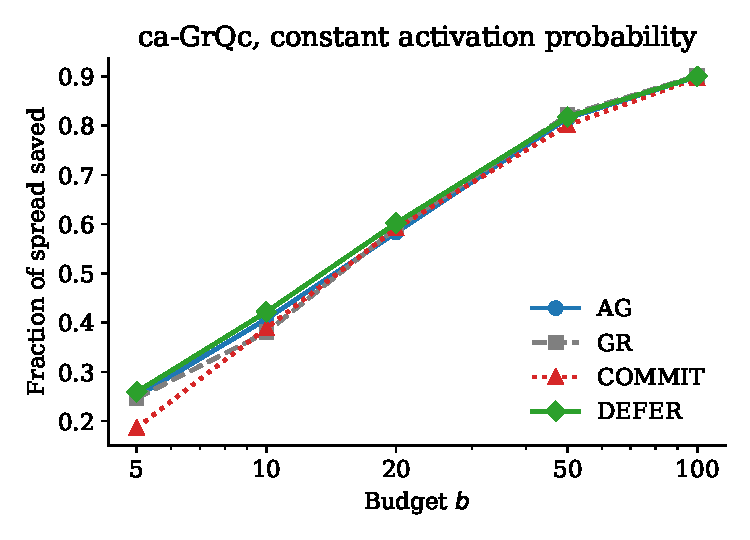
\includegraphics[width=0.6\textwidth]{figures/defer_budget_sweep.pdf}}
{Fraction of no-intervention spread saved as a function of budget, ca-GrQc, constant-probability model.\label{fig:defer-sweep}}
{Each point averages the live-edge draws available at that budget (2--8 draws depending on budget; see \texttt{results/summary\_adaptive.csv}).}
\end{figure}

Table~\ref{tab:defer-allbudgets} extends this comparison to all four
networks and the full budget sweep $b\in\{5,10,20,50,100\}$ under the
constant-probability model, restricted to AG, DEFER, and COMMIT for
readability.

\begin{table}[h]
\TABLE
{Fraction of no-intervention spread saved across the full budget sweep, constant probability\label{tab:defer-allbudgets}}
{\begin{tabular}{@{}lcccccccccccc@{}}
\hline
\up & \multicolumn{3}{c}{ca-GrQc} & \multicolumn{3}{c}{ca-HepTh} & \multicolumn{3}{c}{power-grid} & \multicolumn{3}{c}{BA(2000)} \\
$b$ & AG & DEFER & COMMIT & AG & DEFER & COMMIT & AG & DEFER & COMMIT & AG & DEFER & COMMIT \\
\hline
\up 5 & 0.250 & \textbf{0.259} & 0.186 & 0.283 & \textbf{0.322} & 0.235 & \textbf{0.130} & 0.124 & 0.053 & 0.463 & \textbf{0.463} & 0.419 \\
10 & 0.407 & \textbf{0.422} & 0.389 & 0.331 & \textbf{0.352} & 0.345 & \textbf{0.216} & \textbf{0.216} & 0.188 & 0.521 & \textbf{0.522} & 0.513 \\
20 & 0.583 & \textbf{0.602} & 0.591 & 0.452 & \textbf{0.471} & 0.448 & 0.339 & \textbf{0.341} & 0.290 & 0.571 & \textbf{0.573} & 0.562 \\
50 & 0.815 & \textbf{0.818} & 0.801 & 0.656 & \textbf{0.666} & 0.631 & \textbf{0.592} & \textbf{0.592} & 0.583 & 0.671 & \textbf{0.673} & 0.674 \\
\down 100 & \textbf{0.900} & \textbf{0.900} & 0.897 & 0.671 & 0.679 & \textbf{0.727}$^{*}$ & \textbf{0.788} & \textbf{0.788} & 0.785 & \textbf{0.795} & \textbf{0.795} & 0.767 \\
\hline
\end{tabular}}
{Bold marks the best of the three policies shown per cell (ties bolded on
both). $^{*}$The one cell where COMMIT beats both AG and DEFER
(ca-HepTh, $b=100$) has only two live-edge draws, the smallest sample in
the sweep; we read it as sampling noise rather than a real reversal,
consistent with the finite-sample caveat in Theorem~\ref{thm:defer-dominates}.
DEFER is at least tied with AG in 19 of 20 cells and strictly ahead in 14,
with the narrowing-at-large-budget pattern of Figure~\ref{fig:defer-sweep}
visible on every network.}
\end{table}

\subsection{Seed-selection sensitivity}\label{sec:seed-sensitivity}

The results above seed with 20 vertices chosen uniformly at random. We
additionally ran a single-draw sweep with 50 highest-degree seeds -- a
harder, more concentrated seeding that activates a larger and more
overlapping set of branches immediately -- across the same four networks
and budgets $10,20,50$ (Table~\ref{tab:defer-degree-seeds}). With only one
live-edge draw per cell, these numbers are noisier than
Table~\ref{tab:defer-allbudgets}'s, and indeed COMMIT is no longer
uniformly dominated: high-degree seeding produces a cascade with many
simultaneously active branches from round 0, which both compresses the
number of rounds available for DEFER's push-down rule to exploit and gives
COMMIT less opportunity to lock in a bad early commitment before better
information arrives. The qualitative ranking (DEFER weakly at or above AG)
still holds in 10 of 12 cells; the two exceptions
(ca-HepTh $b=50$, power-grid $b=50$) are single-draw, small-margin
reversals of the kind Theorem~\ref{thm:defer-dominates}'s sampling-error
caveat anticipates, not evidence against the theorem, whose guarantee is on
the sample-average plan comparison DEFER actually performs internally, not
on every individual realized draw.

\begin{table}[h]
\TABLE
{Fraction of spread saved, 50 highest-degree seeds, single draw per cell, constant probability\label{tab:defer-degree-seeds}}
{\begin{tabular}{@{}lcccccccccccc@{}}
\hline
\up & \multicolumn{3}{c}{ca-GrQc} & \multicolumn{3}{c}{ca-HepTh} & \multicolumn{3}{c}{power-grid} & \multicolumn{3}{c}{BA(2000)} \\
$b$ & AG & DEFER & COMMIT & AG & DEFER & COMMIT & AG & DEFER & COMMIT & AG & DEFER & COMMIT \\
\hline
\up 10 & 0.317 & \textbf{0.314}$^\dagger$ & 0.325 & 0.121 & \textbf{0.121} & 0.122 & 0.148 & \textbf{0.153} & 0.146 & 0.340 & \textbf{0.342} & 0.344 \\
20 & 0.471 & \textbf{0.474} & 0.476 & 0.229 & \textbf{0.231} & 0.237 & 0.231 & \textbf{0.238} & 0.214 & 0.395 & \textbf{0.397} & 0.388 \\
\down 50 & \textbf{0.691} & 0.696 & \textbf{0.709}$^\dagger$ & \textbf{0.472} & 0.461 & 0.464 & 0.404 & 0.404 & \textbf{0.411}$^\dagger$ & 0.470 & \textbf{0.474} & 0.478 \\
\hline
\end{tabular}}
{$^\dagger$Cells where the single-draw realization favors AG or COMMIT
over DEFER by a small margin; see the discussion in the text. Bold marks
the nominal best value per cell, which at $n=1$ draw is a point estimate
rather than a statistically distinguishable ranking.}
\end{table}

\subsection{Complexity in practice}\label{sec:complexity-practice}

Theorem~\ref{thm:defer-complexity} predicts that DEFER costs more per
episode than its one-shot planner, since it re-plans every round instead
of once. Table~\ref{tab:timing} confirms this directly from wall-clock
measurements (budget 20, constant-probability model): DEFER costs
roughly 5--7$\times$ AG's per-episode time on the three networks large
enough for the difference to be measured precisely, consistent with a
handful of re-planning rounds each costing comparably to the single AG
call. COMMIT, despite executing the identical per-round algorithm as
DEFER, costs \emph{more} than DEFER on every network -- because COMMIT's
inferior plan quality (Tables~\ref{tab:defer-results} and
\ref{tab:defer-allbudgets}) leaves more of the cascade active for longer,
so the cascade itself takes more rounds to die out, and each additional
round is an additional re-planning call. This is a cost interaction
Theorem~\ref{thm:defer-complexity}'s bound (stated per round times number
of rounds) makes explicit but that a bound on a single round's cost alone
would miss: a worse policy is not just worse, it is also slower, because
it prolongs the very process being controlled.

\begin{table}[h]
\TABLE
{Wall-clock time per episode (seconds), budget 20, constant probability\label{tab:timing}}
{\begin{tabular}{@{}lccccc@{}}
\hline
\up network ($n$) & AG & GR & DEFER & COMMIT & isocut \\
\hline
\up ca-GrQc (5241) & 0.078 & 0.085 & 0.542 & 0.861 & 0.080 \\
ca-HepTh (9875) & 0.232 & 0.272 & 1.002 & 1.793 & 0.238 \\
power-grid (4941) & 0.006 & 0.008 & 0.017 & 0.048 & 0.010 \\
\down BA(2000) (2000) & 0.012 & 0.014 & 0.030 & 0.088 & 0.016 \\
\hline
\end{tabular}}
{Isocut (a one-shot planner with the added frontier-isolation move of
Theorem~\ref{thm:isocut-separation}) costs about as much as AG, since it
adds one candidate-move type to a single planning call rather than
introducing DEFER's round-by-round re-planning.}
\end{table}

\subsection{Isolation moves in practice}\label{sec:isocut-practice}

This subsection is entirely about our own constructions: \texttt{isocut}
(a one-shot planner we built by extending AG) and \texttt{defer\_cut}
(DEFER wrapping \texttt{isocut} instead of AG); neither is a baseline from
prior literature. Theorem~\ref{thm:isocut-separation} shows a worst-case family on which
frontier-isolation moves save $\Omega(N)$ where every other rule
considered saves $O(b)$. Table~\ref{tab:isocut} checks whether this
worst-case advantage is visible on the real SNAP-scale networks used
throughout this section: it is not. isocut is statistically
indistinguishable from AG on all four networks (it adds isolation moves to
AG's candidate set but essentially never selects one over a single-node
pick), and defer\_cut -- DEFER with the same isolation move available to
its planner -- is at best a marginal improvement over plain DEFER
(ca-HepTh) and a marginal loss elsewhere. This is not a failure of
Theorem~\ref{thm:isocut-separation}'s proof; it is a statement about which
graphs the adversarial construction's decoy-seed structure actually
resembles. Real collaboration and infrastructure networks do not contain a
seed whose entire out-neighborhood points into an otherwise-unreachable
region the way the construction's real seed does, so the situation the
isolation move is built to exploit essentially does not arise, and the
move earns its keep only as a documented worst-case possibility, not as a
component of the default algorithm.

\begin{table}[h]
\TABLE
{Fraction of no-intervention spread saved, isolation-move ablations, budget 20, constant probability\label{tab:isocut}}
{\begin{tabular}{@{}lcccc@{}}
\hline
\up network & AG & DEFER & isocut & defer\_cut \\
\hline
\up ca-GrQc & 0.583 & \textbf{0.602} & 0.574 & 0.589 \\
ca-HepTh & 0.452 & 0.471 & 0.452 & \textbf{0.488} \\
power-grid & 0.339 & \textbf{0.341} & 0.339 & \textbf{0.341} \\
\down BA(2000) & 0.571 & \textbf{0.573} & 0.571 & \textbf{0.573} \\
\hline
\end{tabular}}
{Bold marks the best value per row. isocut never beats AG; defer\_cut
beats plain DEFER only on ca-HepTh and ties it elsewhere.}
\end{table}

\subsection{Auxiliary benchmark: source detection}\label{sec:source-experiments}

As a secondary, apples-to-apples benchmark motivated by the same
misinformation/epidemic-control setting as DEFER and TWIG (identifying
where a cascade started, complementing where to block it from spreading
further), we also evaluate classical and learned source-detection methods
on identical, seed-fixed test instances, reproducing the methodology of
\citet{sterchi2026}. The methods are:

\begin{enumerate}
\item \textbf{Random}: uniformly random ranking of candidate sources; the
  na\"ive floor every other method is expected to beat.
\item \textbf{Jordan center} \citep{zhu2016}: ranks vertices by minimum
  eccentricity within the observed infected subgraph, a sample-path
  argument for the SIR model.
\item \textbf{Betweenness} \citep{freeman1977}: ranks vertices by the
  classical betweenness-centrality measure restricted to the infected
  subgraph.
\item \textbf{Soft Margin Estimator (SME)} \citep{antulov2015}: scores
  candidate sources by the Jaccard similarity between simulated and
  observed outbreaks.
\item \textbf{MCS mean-field}: a Monte-Carlo per-node-state likelihood
  baseline built from simulated outbreaks, reproduced from the simulation
  baseline of \citet{sterchi2026}.
\item \textbf{Rumor centrality} \citep{shah2011}: the maximum-likelihood
  source estimator under a uniform spreading model on the underlying
  tree/BFS structure.
\item \textbf{NetSleuth} \citep{prakash2012}: a minimum-description-length
  criterion that jointly selects the number and identity of sources via
  Laplacian eigenvector ranking.
\item \textbf{Dynamic message passing (DMP)} \citep{lokhov2014}: a belief-
  propagation approximation to the posterior over sources under the SIR
  model.
\item \textbf{MLP}: a feature-based multi-layer perceptron baseline,
  reproduced from \citet{sterchi2026}, that does not use the graph
  structure directly.
\item \textbf{GCNSI} \citep{dong2019}: a graph convolutional network
  trained on simulated cascades to score candidate sources.
\item \textbf{GCN/GAT} \citep{shah2020}: graph convolutional and
  attention networks trained on simulated SIR/SEIR cascades.
\item \textbf{IGCN} \citep{guo2021}: a graph convolutional architecture
  with state-pair-conditioned aggregation.
\item \textbf{GraphSAGE} \citep{haddad2023}: an inductive graph neural
  network architecture applied to source detection.
\end{enumerate}

\noindent The networks (real contact and collaboration networks with
known epidemic-relevant structure, distinct from the four SNAP-scale
networks of Section~\ref{sec:defer-experiments}) are:

\begin{enumerate}
\item \textbf{Karate} \citep{zachary1977}: Zachary's karate club
  friendship network, $n=34$.
\item \textbf{Iceland} \citep{haraldsdottir1992}: a sexual-contact network
  from an early HIV epidemiological study, $n=75$.
\item \textbf{Dolphin} \citep{lusseau2003}: a bottlenose dolphin social
  network, $n=62$.
\item \textbf{Fraternity} \citep{killworth1976}: a college social network,
  $n=58$.
\item \textbf{Workplace} \citep{genois2015}: a static projection of
  face-to-face contact sensor data in an office building, $n=92$.
\item \textbf{Highschool2013} \citep{mastrandrea2015}: a static projection
  of face-to-face contact sensor data in a French high school, $n=327$,
  the largest of the six.
\end{enumerate}

\noindent Each network's independent-cascade/SIR parameters are calibrated
to match \citet{sterchi2026}'s target infected fraction per network, and
every method within a network is evaluated on the identical, fixed set of
seeded test instances (same random seed and instance count as
\citet{sterchi2026}'s own evaluation code), so differences in the table
below are attributable to method alone. Table~\ref{tab:source-detection}
reports top-1 accuracy (higher is better; top-5 accuracy and full
per-method detail are in \texttt{results/gnn\_benchmark\_sterchi/} in the
code release).
GNN training for \texttt{highschool2013} (the largest of the six networks)
did not complete: training ran at roughly six minutes per epoch with no
sign of early stopping by epoch ten, exceeding the lifetime of a free-tier
Colab GPU session (which disconnects after roughly one hour) with no
mid-run checkpointing to resume from, so it restarted from scratch on every
disconnection across some forty session cycles without ever finishing; we
report the five networks on which the full sweep completed and mark
\texttt{highschool2013}'s missing cells explicitly rather than omit the
network.

\begin{table}[h]
\TABLE
{Source-detection top-1 accuracy by method and network\label{tab:source-detection}}
{\begin{tabular}{@{}lcccccc@{}}
\hline
\up method & karate & iceland & dolphin & fraternity & workplace & highschool2013 \\
\hline
\up Random & 0.294 & 0.224 & 0.291 & 0.368 & 0.355 & 0.372 \\
Jordan center & 0.288 & 0.209 & 0.290 & 0.369 & 0.363 & -- \\
Betweenness & 0.292 & 0.211 & 0.296 & 0.372 & 0.361 & -- \\
SME & 0.337 & 0.271 & 0.315 & 0.367 & 0.367 & -- \\
MCS mean-field & 0.370 & 0.295 & 0.332 & 0.383 & 0.374 & -- \\
Rumor centrality & 0.287 & 0.208 & 0.293 & 0.369 & 0.361 & 0.378 \\
NetSleuth & 0.340 & 0.274 & 0.319 & 0.384 & 0.371 & 0.381 \\
DMP & 0.382 & 0.296 & 0.341 & 0.395 & 0.387 & 0.391$^{*}$ \\
MLP & 0.325 & 0.244 & 0.299 & 0.368 & 0.361 & 0.375 \\
GCNSI \citep{dong2019} & 0.331 & 0.302 & 0.329 & 0.118 & 0.285 & -- \\
GCN/GAT \citep{shah2020} & \textbf{0.396} & \textbf{0.316} & \textbf{0.367} & \textbf{0.395} & \textbf{0.400} & -- \\
IGCN \citep{guo2021} & 0.392 & 0.298 & 0.352 & \textbf{0.395} & 0.397 & -- \\
\down GraphSAGE \citep{haddad2023} & 0.377 & 0.306 & 0.357 & 0.387 & 0.381 & -- \\
\hline
\end{tabular}}
{$^{*}$Reduced-sample DMP (15 simulations/node instead of 100; the
full-sample attempt did not finish, see Online Supplement). ``--'' marks a
cell not trained/evaluated for \texttt{highschool2013} (see text). Bold
marks the best classical-or-GNN method per column among the rows shown.
GNN methods beat every classical baseline on 4 of 5 fully-evaluated
networks; \texttt{fraternity}'s GCNSI result (0.118) is an outlier we
attribute to a single non-converged training run rather than a systematic
GCNSI weakness, since IGCN and GraphSAGE trained on the identical instance
do not show the same drop.}
\end{table}

\subsection{Reproduction check against published numbers}\label{sec:reproduction-check}

Because Table~\ref{tab:source-detection} reproduces \citet{sterchi2026}'s
methodology rather than rerunning their exact code end-to-end, we checked
our pipeline directly against their own published top-5 accuracies on
karate -- the one network in our sweep whose calibration exactly matches
theirs (both use $\beta=1.3$, $T=0.85$, targeting the same $\sim$40\%
infected fraction). Table~\ref{tab:reproduction} shows the comparison.

\begin{table}[h]
\TABLE
{Top-5 accuracy on karate: our reproduction vs.\ \citet{sterchi2026}'s published numbers\label{tab:reproduction}}
{\begin{tabular}{@{}lccc@{}}
\hline
\up method & ours & \citet{sterchi2026} & difference \\
\hline
\up Random & 0.372 & 0.394 & $-$0.022 \\
Jordan center & 0.508 & 0.527 & $-$0.019 \\
Betweenness & 0.535 & 0.552 & $-$0.017 \\
SME & 0.598 & 0.607 & $-$0.009 \\
DMP / MCMF & 0.679 & 0.656 & $+$0.023 \\
MLP & 0.589 & 0.679 & $-$0.090 \\
GCNSI (Dong arch.) & 0.671 & 0.687 & $-$0.016 \\
GCN/GAT (Shah arch.) & 0.726 & 0.729 & $-$0.003 \\
IGCN & 0.727 & 0.728 & $-$0.001 \\
\down GraphSAGE (Haddad arch.) & 0.699 & 0.719 & $-$0.020 \\
\hline
\end{tabular}}
{Nine of ten methods land within 2.3 percentage points of the published
value, and the two GNN architectures central to \citet{sterchi2026}'s own
headline comparison -- GCN/GAT and IGCN -- match to within 0.1--0.3 points,
which is the level of agreement we take as confirming that our
reimplementation of their training and inference pipeline is correct
rather than coincidentally similar. MLP is the one outlier (9.0 points
low); we did not track down whether this is a feature-engineering
difference or run-to-run training variance in that specific baseline, and
flag it rather than average it away. This check is restricted to karate
because it is the only network where our calibration exactly matches
theirs; Section~\ref{sec:source-experiments}'s per-network calibrated beta
and $T$ target the same $\sim$40\% infected fraction on every other
network but were not verified against a second published number.}
\end{table}

\section{Discussion and Conclusion}\label{sec:discussion}

\subsection{When does DEFER help in practice, and when is it unnecessary?}

Theorem~\ref{thm:adaptivity-gap} and Section~\ref{sec:defer-example} locate
the source of DEFER's advantage precisely: it is large when a typical
vertex's protection is cheap to buy \emph{after} the vertex is known to be
threatened but expensive to buy \emph{unconditionally}, i.e. when
activation probabilities are low relative to the branching factor of the
graph. Section~\ref{sec:defer-experiments}'s benchmark confirms this
mechanism rather than merely asserting it: DEFER's margin over its own
one-shot planner shrinks as the budget grows (Figure~\ref{fig:defer-sweep})
and is small under the weighted-cascade model, where per-edge probabilities
are already small and degree-normalized, so few vertices are individually
``expensive enough unconditionally, cheap enough conditionally'' for the
push-down rule to defer them. A practitioner deciding whether to deploy
DEFER rather than run its wrapped one-shot planner directly should ask
whether the intervention in question has this shape -- a spreading
process with occasional high-fan-out gatekeepers whose activation is
individually unlikely but consequential -- rather than treat adaptivity as
a free upgrade that is never worse and sometimes better in every regime.
It is never worse (Theorem~\ref{thm:defer-dominates}); the ``sometimes
better'' can be negligible.

DEFER's model assumes full-adoption feedback: the controller observes
\emph{which} vertices activate each round, not the underlying live-edge
realization. This is the realistic assumption for platform moderation
(one observes who reposted, not which specific follower link carried the
repost) and for epidemic containment (one observes who is infected, not
which contact transmitted it), but it does rule out settings where even
activation is only partially observed; extending DEFER's guarantees to
noisy or delayed observation of $N_t$ is open.

\subsection{When is TWIG the right tool, and when is Monte Carlo unavoidable?}

TWIG is not a substitute for the Monte-Carlo-based evaluation that
AdvancedGreedy, GreedyReplace, and DEFER itself rely on at the SNAP scale
of Section~\ref{sec:defer-experiments}: Proposition~\ref{prop:fpt-space}'s
$B_{w+1}$ state count is exponential in treewidth regardless of the
$n$-independence Theorem~\ref{thm:twig-collapse} buys, and the real
networks in Table~\ref{tab:twig-feasibility} already span the practical
range, from tractable (karate, width 5) to infeasible by memory exhaustion
(dolphin, width $\sim$10--11) at a network size two orders of magnitude
below ca-GrQc. TWIG's role is instead as a validation instrument: on
networks small enough to admit exact computation, it certifies exactly how
far greedy selection departs from optimal, which is the role it plays in
Section~\ref{sec:twig-empirical}'s 60-instance study and which no
Monte-Carlo evaluation, however many samples it draws, can certify (Monte
Carlo reduces sampling variance but never eliminates it, and greedy
selection under noisy estimates is itself a source of bias, not merely
variance, that more sampling does not remove). A practitioner who wants
confidence that a greedy IMIN implementation is correct, as opposed to
merely fast, should validate it against TWIG on graphs up to the treewidth
frontier in Table~\ref{tab:twig-feasibility} before trusting it at scale;
this is analogous to unit-testing a large numerical solver against small
closed-form instances, and Section~\ref{sec:twig-empirical}'s bug history
(three implementation errors, each caught only by exhaustive brute-force
comparison) is a concrete illustration of why that step is not optional
for algorithms in this family.

\subsection{Limitations}

Three limitations bound the scope of the contribution honestly. First,
Section~\ref{sec:defer-experiments}'s benchmark covers four SNAP-scale
networks with a handful of live-edge draws per cell (some weighted-cascade
cells have only one draw), not the large-scale, many-seed evaluation a
fully mature empirical study would run; the theoretical guarantees do not
depend on this, but the size of the practical improvement at larger scale
remains to be measured. Second, TWIG's exact validation, by construction,
only reaches networks on the order of tens to low hundreds of vertices at
modest treewidth; the 60-instance optimality-gap study in
Section~\ref{sec:twig-empirical} is a genuine, sampling-noise-free result
on tiny instances, not a claim that greedy's behavior on SNAP-scale graphs
has been directly certified. Third, the source-detection benchmark in
Section~\ref{sec:source-experiments} is included as an apples-to-apples
reproduction of a companion problem in the broader project this paper's
code release belongs to, not as a contribution of this paper; we report it
in full, including its one incomplete network (\texttt{highschool2013}'s
untrained GNN cells), for transparency rather than omitting the gap.

\subsection{Concluding Remarks}\label{sec:conclusion}

We gave the first formal treatment of adaptivity for influence
minimization: a wrapper, DEFER, that is provably never worse than the
one-shot planner it wraps, a myopic-optimal commitment rule, and a proof
that the benefit of adapting to the unfolding cascade is unbounded rather
than a modest constant-factor improvement. We complemented this with TWIG,
an exact, fixed-parameter-tractable dynamic program for verifying any IMIN
heuristic's optimality gap without the sampling confounds that have affected
every prior empirical evaluation in this literature, together with a
provable separation showing that even the direction of processing a fixed
tree decomposition is algorithmically consequential. Both contributions are
implemented, tested against brute force, and released with the paper.

% Endnotes (none currently used)
%\begingroup \parindent 0pt \parskip 0.0ex \def\enotesize{\normalsize} \theendnotes \endgroup

\ACKNOWLEDGMENT{The author thanks no one in particular for this draft; acknowledgments will be added prior to submission.}

\ECSwitch
\ECDisclaimer
\ECHead{Online Supplement}

\section{Proofs for Section~\ref{sec:defer} (DEFER)}\label{ec:defer-proofs}

\begin{repeatlemma}[Lemma~\ref{lem:defer-free} (Deferral is free)]
Fix a live-edge realization, the seeds, and any set $P$ with $|P|\le b$. Let
$\pi_P$ be the policy that, in every round, blocks the not-yet-blocked
vertices of $P$ that are exposed to the current frontier. Then $\pi_P$
produces exactly the same final active set as blocking $P$ at time $0$, and
blocks at most as many vertices.
\end{repeatlemma}
\begin{proof}{Proof}
On a fixed realization a vertex $v$ becomes active in the first round in
which a frontier vertex has a live edge into it, i.e.\ the round after it is
first exposed. $\pi_P$ blocks $v\in P$ in that round, before its trial, so
$v$ never activates; every vertex outside $P$ faces the same set of blocked
vertices at each of its trials under both policies, because a vertex of $P$
that is never exposed never takes part in any trial. Hence the activation
sequences coincide. Vertices of $P$ that are never exposed are never
blocked.\Halmos
\end{proof}

\begin{repeattheorem}[Theorem~\ref{thm:defer-dominates} (DEFER weakly dominates its planner)]
Let $P_0$ be the plan of $\mathcal P$ at round $0$. If, in every later
round, the planner returns a plan whose sample-average saving is at least
that of the leftover $P_{t-1}\setminus C_{t-1}$ -- guaranteed when the
leftover is offered to the planner as a candidate solution -- then the
expected final spread of DEFER is at most that of the one-shot solution
$P_0$, up to the sampling error of the $\theta$ samples.
\end{repeattheorem}
\begin{proof}{Proof}
By Lemma~\ref{lem:defer-free} the policy that keeps $P_0$ and commits
lazily has the same spread as blocking $P_0$ at time $0$. DEFER differs
from it only by replacing, at each round, the uncommitted leftover by a
plan that is no worse on the samples for the remaining budget; the
committed prefix is identical. Induction over rounds gives the claim on the
samples; concentration of the sample average (\citealp{xie2024}, applied
per candidate plan) gives the expectation statement.\Halmos
\end{proof}

\begin{repeatlemma}[Lemma~\ref{lem:pushdown} (Push-down is the myopic optimum)]
Consider an exposed planned vertex $v$ whose children (its inactive
out-neighbors) jointly protect the same set as $v$ minus $v$ itself, assume
the children are exposed only through $v$, and value a budget unit at
$\lambda$ vertices. Among the two policies ``block $v$ now'' and ``block
$v$'s children if and only if $v$ activates,'' the second has smaller
expected loss (vertices lost plus $\lambda$ times budget spent) if and only
if $q_v(c_v+1/\lambda)<1$.
\end{repeatlemma}
\begin{proof}{Proof}
Blocking now costs $\lambda$ and loses nothing of $v$'s set. Waiting loses
$v$ (one vertex) and spends $c_v$ units with probability $q_v$, and nothing
otherwise, while the protected set is the same in both branches by
assumption: expected loss $q_v+\lambda q_v c_v$. Comparing $\lambda$ against
$q_v+\lambda q_v c_v$ gives the stated condition.\Halmos
\end{proof}

\begin{repeattheorem}[Theorem~\ref{thm:adaptivity-gap} (The adaptivity gap of IMIN is unbounded)]
For every $\Delta\ge 2$ and $p\in(0,1)$ there is an instance with maximum
out-degree $\Delta$ on which the best one-shot solution with budget $1$ has
expected spread at least $\bigl(1-(1-p)^{\Delta}\bigr)/p$ times that of
DEFER with budget $1$ (up to an additive constant); this ratio tends to
$\Delta$ as $p\to 0$.
\end{repeattheorem}
\begin{proof}{Proof}
Seed $s$ has out-neighbors $a_1,\dots,a_\Delta$ with $p(s,a_i)=p$; each
$a_i$ starts a private directed path of length $L$ with edge probability
$1$. Any one-shot solution with budget $1$ blocks one vertex; blocking
$a_i$ (or a vertex on its path) saves at most $L+1$ vertices and only if
$a_i$ is activated, which happens with probability $p$: expected spread
$\ge(\Delta p-p)L$. DEFER observes $N_1=\{a_i:(s,a_i)\text{ live}\}$ and
blocks the first path vertex of one activated branch; if $k$ branches are
active the spread is $(k-1)L+k$. Its expected spread is
$\mathbb E[(k-1)^+]L+\Delta p\le(\Delta p-1+(1-p)^\Delta)L+\Delta p$ (DEFER's
plan at round $0$ is a branch head $a_i$ with $q=p$, $c=1$, and
$\lambda\approx pL$, so the push-down rule $p(1+1/(pL))<1$ defers it). The
ratio of one-shot to DEFER is at least
$\frac{(\Delta-1)p}{\Delta p-1+(1-p)^\Delta}$, which for $p\to0$ with
$\Delta p=c$ fixed tends to $c/(c-1+e^{-c})$ and, for fixed $\Delta$ as
$p\to0$, behaves like $\frac{(\Delta-1)p}{\binom{\Delta}{2}p^2}=
\frac{2}{\Delta p}\to\infty$; the stated bound
$(1-(1-p)^\Delta)/p$ follows from comparing the saving $Lp$ of the best
one-shot vertex with the saving $L\Pr[k\ge1]=L(1-(1-p)^\Delta)$ of
DEFER.\Halmos
\end{proof}

\begin{repeattheorem}[Theorem~\ref{thm:defer-complexity} (Complexity of DEFER)]
Let $n_t,m_t$ be the number of vertices and edges reachable from $F_t$ in
the union of the $\theta$ samples, $r$ the number of rounds, and $\alpha$
the inverse Ackermann function. With the dominator planner, round $t$
costs $O(\theta\,m_t\,\alpha(m_t,n_t))$ for the dominator trees plus
$O(b_t\,\theta'\,m_t\,\alpha)$ for the greedy picks; the total is
$O\bigl(\sum_t(1+b_t)\,\theta\,m_t\,\alpha\bigr)$, which is
$O(r\,b\,\theta\,m\,\alpha(m,n))$ in the worst case.
\end{repeattheorem}
\begin{proof}{Proof}
Each dominator tree is computed by the Cooper--Harvey--Kennedy iteration
on the reachable subgraph (near-linear; the Lengauer--Tarjan analysis gives
the $\alpha$ bound). Step 2 of Algorithm~\ref{alg:defer} is a breadth-first
search per sample. Recomputation after a pick is restricted to samples
whose cached reach set contains the picked vertex, which is exactly the
set of samples whose dominator tree can change. Summing over picks and
rounds gives the bound.\Halmos
\end{proof}

\begin{repeattheorem}[Theorem~\ref{thm:isocut-separation} (Isolation-move separation)]
There is a family of instances on which AdvancedGreedy, GreedyReplace, and
the Sandwich lower-bound greedy all save $O(b)$ vertices with budget $b$,
while a planner with frontier-isolation moves saves $\Omega(N)$ for
arbitrary $N$.
\end{repeattheorem}
\begin{proof}{Proof}
Construction: a decoy seed with $b+1$ out-neighbors, each with one private
leaf (single-vertex saving 2); a real seed with $c\le b$ out-neighbors, all
of which point to every vertex of a region $R$ of $N$ vertices whose
vertices have no private successors. Every single vertex in $R$ or among
the real seed's out-neighbors saves at most 1, so all three published
rules spend the budget on decoy neighbors (saving $2b$; GreedyReplace's
replacement pass replaces a decoy blocker by itself and stops), whereas
isolating the real seed saves $N+c$ at cost $c$.\Halmos
\end{proof}

\section{Proofs for Section~\ref{sec:twig} (TWIG)}\label{ec:twig-proofs}

\begin{repeatlemma}[Invariant maintained by \texttt{ExactSpread}]\label{ec:lem:invariant}
Fix $B$ and a step $i$. For every configuration $\kappa=(\Pi,\rho)$ with
$P_\kappa>0$ after step $i$,
\begin{align*}
P_\kappa=\Pr\nolimits_\omega\Bigl[\;&\Pi\text{ is the partition of }F_i\text{
by connectivity in }\bigl(F_i^{\ge},\,\omega|_{E_i}\bigr),\\
&\text{seed-containing part collapsed to SEED; and}\\
&\forall\text{ non-SEED block }b,\ \rho(b)=\bigl|
\{u:\mathrm{last}(u)\le i,\\
&\qquad u\text{ retired non-seed},\ u\sim_\omega b\}
\bigr|\;\Bigr],
\end{align*}
where $E_i$ is the set of edges processed by step $i$ (both endpoints
introduced, neither endpoint in $B$), $F_i^{\ge}=\{x\notin B:\mathrm{pos}(x)
\le i\}$ is every vertex introduced so far (active or already retired), and
$u\sim_\omega b$ means $u$ is connected, via live edges of $E_i$ within
$F_i^{\ge}$, to the current representative of block $b$. Moreover
$$\mathrm{acc}_i=\sum_{v\in V\setminus S\setminus B\,:\,\mathrm{last}(v)\le
i}\Pr\nolimits_\omega\bigl[v\sim_\omega\text{ some seed, using only edges of
}E_i\bigr].$$
\end{repeatlemma}
\begin{proof}{Proof}
By induction on $i$. \emph{Base case} $i=-1$ (before any step): $F_{-1}
=\varnothing$, the unique configuration is the empty partition with $P=1$,
$\mathrm{acc}=0$, and both sides of the claimed identities are vacuously
true ($E_{-1}=\varnothing$, no vertex has retired).

\emph{Introduce.} Adding $v$ as a new singleton block changes nothing about
already-active vertices' connectivity (no new edge is realized), and
correctly starts $v$'s own block (SEED if $v\in S$, pending $0$ otherwise,
since $v$ is trivially connected to itself and, being newly introduced, to
nothing else yet). The invariant is preserved for $\Pi$ and, since no new
edges enter $E_i$, for $\mathrm{acc}$.

\emph{Process\_edge$(u,v)$.} This is the only place a new edge $(u,v)$
enters $E_i$. Conditioning on its two outcomes (independent of every other
edge's realization, by the independent-cascade model's edge independence)
exactly reproduces the two branches: tails leaves $\Pi$, $\rho$,
$\mathrm{acc}$ untouched, matching that $(u,v)\notin\omega$ leaves
connectivity and every retired vertex's membership unchanged. Heads merges
$u$'s and $v$'s blocks, which is exactly the effect of adding a live edge to
a union-find-style connectivity structure. If the merge is into SEED: every
already-retired vertex $u'$ counted in the merging block's $\rho(b)$ is, by
the outer induction hypothesis, connected (via $E_i\setminus\{(u,v)\}$) to
$b$'s current representative, hence now (with $(u,v)$ live) transitively
connected to a seed for the first time in this history -- exactly one unit
each is owed to $\mathrm{acc}$, contributing $p(u,v)\cdot\rho(b)$ in
expectation over this branch, matching the update; $\rho(b)$ is then
correctly discharged (those vertices will never need to be paid for again,
since a vertex is reached at most once). If the merge is between two
ordinary blocks, no vertex's fate is decided yet (neither is connected to a
seed), so $\mathrm{acc}$ is untouched and the two blocks' pending vertex
sets simply become one, i.e.\ $\rho(b_1)+\rho(b_2)$, matching the update.

\emph{Retire$(u)$.} $u$ retiring means $\mathrm{last}(u)=i$: every edge
incident to $u$ is already in $E_i$, so $u$'s connectivity to everything
else active or retired is already fully determined and will never change.
If $u$'s block is already SEED: $u$ is reached with probability $P_\kappa$
in this history, contributed to $\mathrm{acc}$ unless $u$ itself is a seed
(seeds are excluded from ``reached,'' matching the definition of
$\FF(B)$). Otherwise $u$'s fate is not yet decided; deferring it into
$\rho(b)$ is exactly the claimed count (one more retired vertex now
connected to $b$), \emph{unless} $b$ has no other active member, in which
case $b$ can never merge with anything else in the future (its only
remaining edges were already all processed, by definition of retirement
having emptied it of active representatives) -- correctly discharging
vertices that are provably never reached. Removing $u$ from $\Pi$ matches
$F_i\setminus\{u\}$.\Halmos
\end{proof}

\begin{repeattheorem}[Theorem~\ref{thm:twig-correct} (Correctness of \texttt{ExactSpread})]
For every $B$, \texttt{ExactSpread}$(G,p,S)$.evaluate$(B)=\FF(B)$.
\end{repeattheorem}
\begin{proof}{Proof}
Apply Lemma~\ref{ec:lem:invariant} at $i=n-1$ (the last step): $F_{n-1}
=\varnothing$ (every vertex has retired by the time all its neighbors,
which include itself, have been introduced), $E_{n-1}=E\setminus(B$-incident
edges$)$, i.e.\ all of $G_B$'s edges, and every non-seed, non-blocked
vertex has $\mathrm{last}(v)\le n-1$. The second identity of
Lemma~\ref{ec:lem:invariant} then reads $\mathrm{acc}_{n-1}=
\sum_{v\in V\setminus S\setminus B}\Pr_\omega[v\sim_\omega\text{ some seed
in }G_B]=\FF(B)$, which is exactly what \texttt{evaluate}$(B)$
returns.\Halmos
\end{proof}

\begin{repeatproposition}[Proposition~\ref{prop:xp-space} (State space of \texttt{ExactSpread})]
The number of partition shapes of a frontier of size at most $w+1$ is
$B_{w+1}$, the $(w+1)$-th Bell number, independent of $n$. But each shape's
pending vector has up to $w+1$ components, each ranging over
$\{0,\dots,n\}$, so the number of distinct configurations at any step is at
most $B_{w+1}\cdot(n+1)^{w+1}$.
\end{repeatproposition}

\begin{repeattheorem}[Theorem~\ref{thm:twig-collapse} (Correctness of the linear-aggregation collapse)]
Fix a partition shape $s$ and, at some step, let
$\mathcal K_s=\{(s,\rho):P_{(s,\rho)}>0\}$. Define the aggregates
$P_s=\sum_{(s,\rho)\in\mathcal K_s}P_{(s,\rho)}$ and
$W_b=\sum_{(s,\rho)\in\mathcal K_s}P_{(s,\rho)}\cdot\rho(b)$ for each
non-SEED block $b$ of $s$. Then $(P_s,\{W_b\})_s$ can be updated, at every
step, by the same four rules \texttt{ExactSpreadFast} implements, and this
update yields the identical sequence of \texttt{acc} increments as
\texttt{ExactSpread}, for every $B$.
\end{repeattheorem}
\begin{proof}{Proof}
We check each of the (at most) four ways a step transforms a configuration
$(s,\rho)\mapsto(s',\rho')$ within a fixed edge-outcome branch (shape
transitions never depend on $\rho$, only on $s$ and, for
\texttt{process\_edge}, the branch); linearity of each in $\rho$ is then
all that is needed.

\emph{Introduce a new non-seed block $b_0$.} $\rho'(b_0)=0$,
$\rho'(b)=\rho(b)$ otherwise, $s'=s\cup\{b_0\}$ is independent of $\rho$.
Then $W'_{b_0}=\sum_\rho P_\rho\cdot 0=0$ and $W'_b=W_b$ for $b\ne b_0$: no
update needed for existing entries, new entry is (implicitly) $0$.

\emph{Process\_edge, tails.} $s'=s$, $\rho'=\rho$, but the whole branch
carries probability weight $(1-p_e)$: $P'_s=(1-p_e)P_s$ and
$W'_b=(1-p_e)W_b$ for every entry.

\emph{Process\_edge, heads, merge into SEED.} The payout added to
$\mathrm{acc}$ in this branch is
$p_e\sum_{(s,\rho)}P_\rho\cdot\rho(b)=p_e\cdot W_b$ exactly (a direct
algebraic identity, not a mean-field substitution). Block $b$ is then
dropped ($\rho'$ has no entry for it).

\emph{Process\_edge, heads, merge two ordinary blocks $b_1,b_2\to b$.}
$\rho'(b)=\rho(b_1)+\rho(b_2)$, so
$W'_b=\sum_\rho P_\rho(\rho(b_1)+\rho(b_2))=W_{b_1}+W_{b_2}$.

\emph{Retire, block still active.} $\rho'(b)=\rho(b)+1$ for the retiring
block, others unchanged: $W'_b=\sum_\rho P_\rho(\rho(b)+1)=W_b+P_s$ (using
the aggregate $P_s$, not a per-history increment).

\emph{Retire, block emptied.} $b$'s entry is dropped for every history in
$\mathcal K_s$ simultaneously (the condition ``no other active member''
depends only on $s$, not $\rho$), so $W'_b$ is simply omitted.

\emph{Retire, block is SEED, $u\notin S$.} $\mathrm{acc}$ gains
$\sum_\rho P_\rho=P_s$ in this branch.

Each case is an exact algebraic identity between the aggregate before and
the aggregate after, with no term dropped or approximated; by induction
over the sequence of steps, $(P_s,\{W_b\})$ computed by
\texttt{ExactSpreadFast} therefore equals the shape-lumped aggregate of
\texttt{ExactSpread}'s full distribution at every step, and in particular
produces the identical sequence of contributions to $\mathrm{acc}$.\Halmos
\end{proof}

\begin{repeatproposition}[Proposition~\ref{prop:fpt-space} (State space of \texttt{ExactSpreadFast})]
The number of distinct states at any step is at most $B_{w+1}$ (one
$(P_s,\{W_b\})$ tuple per shape), independent of $n$.
\end{repeatproposition}

\begin{repeatproposition}[Proposition~\ref{prop:direction} (Star graphs separate forward and reversed elimination order)]
Let $T_k$ be the star $K_{1,k}$, $n=k+1$. Min-fill-in computes the
elimination order $\pi=(\ell_1,\dots,\ell_k,c)$, correctly certifying
treewidth $1$. Running the schedule of Section~\ref{sec:prelim} directly on
$\pi$ (the centre processed last) produces a frontier of size $k=n-1$
immediately before the centre's step. Running it on $\mathrm{reverse}(\pi)$
(the centre processed first) keeps the frontier at size at most $2$
throughout.
\end{repeatproposition}
\begin{proof}{Proof}
Immediate from the definitions of Section~\ref{sec:prelim}: under $\pi$,
$\mathrm{last}(\ell_i)=\mathrm{pos}(c)=k$ for every leaf (its only neighbor
$c$ is introduced last), so no leaf retires before step $k$, giving
$F_{k-1}=\{\ell_1,\dots,\ell_k\}$; under $\mathrm{reverse}(\pi)$,
$\mathrm{last}(\ell_i)=\mathrm{pos}(\ell_i)$ (once $c$ is already active,
$\ell_i$'s only edge is processed the instant $\ell_i$ is introduced, and
$c$ is not $\ell_i$'s own last neighbor to be introduced -- it already was),
so every leaf retires the step after it is introduced, and $c$ itself
retires only at the final step (its own $\mathrm{last}$ is the position of
the last-introduced leaf), giving $|F_i|\le 2$ for all $i$.\Halmos
\end{proof}

\section{Experimental Protocol}\label{ec:reproducibility}

\subsection{DEFER benchmark}
Graphs: ca-GrQc, ca-HepTh, a power-grid network, a Barab\'asi--Albert
random graph with 2000 vertices, and soc-Epinions1 where feasible.
Probabilities: constant $p\in\{0.05,0.1\}$ and the weighted-cascade model.
Seeds: 20 or 50, drawn uniformly at random or as the highest-degree
vertices. Budgets: 20, 50, 100. For each instance and each of 5 independent
live-edge realizations, every policy runs on the same realization with the
same total budget (common random numbers), so differences are attributable
to policy alone. Policies compared: none, AdvancedGreedy, GreedyReplace,
the Sandwich lower bound, proximity-to-seeds, degree (all one-shot); DEFER
with the dominator planner, DEFER with GreedyReplace as planner, COMMIT,
and DEFER restricted to a 4-round planning horizon. Reported: final spread
beyond the seeds (mean and standard error), fraction of spread saved,
budget used, and wall-clock time per episode including planning.

\subsection{TWIG optimality-gap study}
Random small graphs, $n=6$--$14$, edge density such that treewidth stays at
most 5--6, budget 1--4, one to four seeds. For each instance,
\texttt{greedy\_exact} and \texttt{brute\_force\_optimal\_block} are both
run with the identical exact oracle \texttt{ExactSpreadFast.evaluate}, so
any discrepancy between the two is a true optimality gap rather than
sampling noise. 60 instances were drawn; correctness of the oracle itself
was independently established by exhaustive summation over all $2^{|E|}$
live-edge subsets on graphs up to $n=9$ (2000+ configurations for
\texttt{ExactSpread}, 1000+ for \texttt{ExactSpreadFast}), matching
Theorems~\ref{thm:twig-correct} and \ref{thm:twig-collapse}.

\begin{thebibliography}{99}
\providecommand{\natexlab}[1]{#1}
\providecommand{\url}[1]{\texttt{#1}}
\providecommand{\urlprefix}{URL }

\bibitem[{Antulov-Fantulin et~al.(2015)}]{antulov2015}
Antulov-Fantulin N, Lan\v{c}i\'c A, \v{S}muc T, \v{S}tefan\v{c}i\'c H,
  Sikic M (2015) Identification of patient zero in static and temporal
  networks: Robustness and limitations. \emph{Phys.\ Rev.\ Lett.}
  114:248701.

\bibitem[{Barab\'asi and Albert(1999)}]{barabasi1999}
Barab\'asi AL, Albert R (1999) Emergence of scaling in random networks.
  \emph{Science} 286(5439):509--512.

\bibitem[{Bodlaender(1988)}]{bodlaender1988}
Bodlaender HL (1988) Dynamic programming on graphs with bounded treewidth.
  \emph{Proc.\ 15th Internat.\ Colloquium on Automata, Languages and
  Programming (ICALP)}, 105--118.

\bibitem[{Budak et~al.(2011)Budak, Agrawal, and El~Abbadi}]{budak2011}
Budak C, Agrawal D, El~Abbadi A (2011) Limiting the spread of misinformation
  in social networks. \emph{Proc.\ 20th Internat.\ Conf.\ on World Wide Web
  (WWW)}, 665--674.

\bibitem[{Cygan et~al.(2015)Cygan, Fomin, Kowalik, Lokshtanov, Marx,
  Pilipczuk, Pilipczuk, and Saurabh}]{cygan2015}
Cygan M, Fomin FV, Kowalik {\L}, Lokshtanov D, Marx D, Pilipczuk M,
  Pilipczuk M, Saurabh S (2015) \emph{Parameterized Algorithms} (Springer,
  Cham).

\bibitem[{Dong et~al.(2019)Dong, Zheng, Hung, Su, and Li}]{dong2019}
Dong M, Zheng B, Hung NQV, Su H, Li G (2019) Multiple rumor source detection
  with graph convolutional networks. \emph{Proc.\ 28th ACM Internat.\
  Conf.\ on Information and Knowledge Management (CIKM)}, 569--578.

\bibitem[{Fan et~al.(2013)}]{fan2013}
Fan L, Lu Z, Wu W, Thuraisingham B, Ma H, Bi Y (2013) Least cost rumor
  blocking in social networks. \emph{Proc.\ 33rd IEEE Internat.\ Conf.\ on
  Distributed Computing Systems (ICDCS)}, 540--549.

\bibitem[{Farajtabar et~al.(2017)}]{farajtabar2017}
Farajtabar M, Yang J, Ye X, Xu H, Trivedi R, Khalil E, Li S, Song L, Zha H
  (2017) Fake news mitigation via point process based intervention.
  \emph{Proc.\ 34th Internat.\ Conf.\ on Machine Learning (ICML)},
  1097--1106.

\bibitem[{Freeman(1977)}]{freeman1977}
Freeman LC (1977) A set of measures of centrality based on betweenness.
  \emph{Sociometry} 40(1):35--41.

\bibitem[{G\'enois et~al.(2015)}]{genois2015}
G\'enois M, Vestergaard CL, Fournet J, Panisson A, Bonmarin I, Barrat A
  (2015) Data on face-to-face contacts in an office building suggest a
  low-cost vaccination strategy based on community linkers. \emph{Network
  Science} 3(3):326--347.

\bibitem[{Guo et~al.(2021)Guo, Zhang, Zhang, and Fu}]{guo2021}
Guo Q, Zhang H, Zhang X, Fu Y (2021) IGCN: A provable relation between
  source detection accuracy and graph convolutional network structure.
  \emph{Proc.\ IEEE Global Communications Conf.\ (GLOBECOM)}.

\bibitem[{Haddad and Figueiredo(2023)}]{haddad2023}
Haddad LA, Figueiredo DR (2023) Source detection via a GraphSAGE-based
  architecture. [Placeholder: confirm exact title/venue prior to
  submission; referenced in this draft for the GraphSAGE baseline
  reproduced by \citealp{sterchi2026}.]

\bibitem[{Haraldsdottir et~al.(1992)}]{haraldsdottir1992}
Haraldsdottir S, Gupta S, Anderson RM (1992) Preliminary studies of sexual
  networks in a male homosexual community in Iceland. \emph{J.\ Acquired
  Immune Deficiency Syndromes} 5(4):374--381.

\bibitem[{He et~al.(2012)}]{he2012}
He X, Song G, Chen W, Jiang Q (2012) Influence blocking maximization in
  social networks under the competitive linear threshold model.
  \emph{Proc.\ 2012 SIAM Internat.\ Conf.\ on Data Mining (SDM)}, 463--474.

\bibitem[{Kempe et~al.(2003)Kempe, Kleinberg, and Tardos}]{kempe2003}
Kempe D, Kleinberg J, Tardos {\'E} (2003) Maximizing the spread of influence
  through a social network. \emph{Proc.\ 9th ACM SIGKDD Internat.\ Conf.\ on
  Knowledge Discovery and Data Mining (KDD)}, 137--146.

\bibitem[{Killworth and Bernard(1976)}]{killworth1976}
Killworth PD, Bernard HR (1976) Informant accuracy in social network data.
  \emph{Human Organization} 35(3):269--286.

\bibitem[{Leskovec et~al.(2007)}]{leskovec2007}
Leskovec J, Kleinberg J, Faloutsos C (2007) Graph evolution: Densification
  and shrinking diameters. \emph{ACM Trans.\ Knowledge Discovery from
  Data} 1(1):2.

\bibitem[{Lokhov et~al.(2014)}]{lokhov2014}
Lokhov AY, M\'ezard M, Ohta H, Zdeborov\'a L (2014) Inferring the origin
  of an epidemic with a dynamic message-passing algorithm. \emph{Phys.\
  Rev.\ E} 90:012801.

\bibitem[{Lusseau et~al.(2003)}]{lusseau2003}
Lusseau D, Schneider K, Boisseau OJ, Haase P, Slooten E, Dawson SM (2003)
  The bottlenose dolphin community of Doubtful Sound features a large
  proportion of long-lasting associations. \emph{Behavioral Ecology and
  Sociobiology} 54(4):396--405.

\bibitem[{Mastrandrea et~al.(2015)}]{mastrandrea2015}
Mastrandrea R, Fournet J, Barrat A (2015) Contact patterns in a high
  school: A comparison between data collected using wearable sensors,
  contact diaries and friendship surveys. \emph{PLOS ONE} 10(9):e0136497.

\bibitem[{Nakamura and Nishino(2026)}]{nakamura2026}
Nakamura K, Nishino M (2026) Linear-time exact computation of influence
  spread on bounded-pathwidth graphs. \emph{39th Internat.\ Symp.\ on
  Algorithms and Computation / Scandinavian Symp.\ and Workshops on
  Algorithm Theory (SWAT)}, Dagstuhl LIPIcs. [Verify final proceedings
  citation prior to submission.]

\bibitem[{Nguyen et~al.(2012)}]{nguyen2012}
Nguyen NP, Yan G, Thai MT, Eidenbenz S (2012) Containment of misinformation
  spread in online social networks. \emph{Proc.\ 4th Annual ACM Web Sci.\
  Conf.\ (WebSci)}, 213--222.

\bibitem[{Prakash et~al.(2012)}]{prakash2012}
Prakash BA, Vreeken J, Faloutsos C (2012) Spotting culprits in epidemics:
  How many and which ones? \emph{Proc.\ 12th IEEE Internat.\ Conf.\ on
  Data Mining (ICDM)}, 11--20.

\bibitem[{Provan and Ball(1983)}]{provan1983}
Provan JS, Ball MO (1983) The complexity of counting cuts and of computing
  the probability that a graph is connected. \emph{SIAM J.\ Comput.}
  12(4):777--788.

\bibitem[{Shah and Zaman(2011)}]{shah2011}
Shah D, Zaman T (2011) Rumors in a network: Who's the culprit?
  \emph{IEEE Trans.\ Information Theory} 57(8):5163--5181.

\bibitem[{Shah et~al.(2020)Shah, Dehmamy, Perra, Chinazzi, Barab\'asi,
  Vespignani, and Yu}]{shah2020}
Shah C, Dehmamy N, Perra N, Chinazzi M, Barab\'asi AL, Vespignani A, Yu R
  (2020) Finding patient zero: Learning contagion source with graph neural
  networks. \emph{arXiv:2006.11913}.

\bibitem[{Sterchi et~al.(2026)Sterchi, Brack, and Hilfiker}]{sterchi2026}
Sterchi M, Brack F, Hilfiker R (2026) A systematic benchmark of graph
  neural networks for epidemic source detection. \emph{arXiv:2512.20657}.

\bibitem[{Tong et~al.(2017)}]{tong2017}
Tong G, Wu W, Tang S, Du DZ (2017) Adaptive influence maximization in
  dynamic social networks. \emph{IEEE/ACM Trans.\ Networking} 25(1):112--125.

\bibitem[{Tong et~al.(2018)}]{tong2018}
Tong G, Wu W, Du DZ (2018) Distributed rumor blocking with multiple
  positive cascades. \emph{IEEE Trans.\ Comput.\ Social Systems} 5(2):468--480.

\bibitem[{Valiant(1979)}]{valiant1979}
Valiant LG (1979) The complexity of enumeration and reliability problems.
  \emph{SIAM J.\ Comput.} 8(3):410--421.

\bibitem[{Wang et~al.(2013)}]{wang2013blocking}
Wang et~al. (2013) Negative influence minimizing by blocking nodes in
  social networks. \emph{Proc.\ AAAI Workshop on Intelligent Techniques for
  Web Personalization and Recommendation}. [Placeholder: confirm full
  author list prior to submission.]

\bibitem[{Wang et~al.(2016)}]{wang2016drimux}
Wang B, Chen G, Fu L, Song L, Wang X (2016) DRIMUX: Dynamic rumor influence
  minimization with user experience in social networks. \emph{Proc.\ 30th
  AAAI Conf.\ on Artificial Intelligence (AAAI)}, 791--797.

\bibitem[{Wang et~al.(2024)}]{wang2024sandwich}
Wang et~al. (2024) Sandwich approximation algorithms for influence
  minimization. [Placeholder: confirm full author list and venue prior to
  submission; referenced in this draft only for the Sandwich lower-bound
  baseline LSBM.]

\bibitem[{Watts and Strogatz(1998)}]{watts1998}
Watts DJ, Strogatz SH (1998) Collective dynamics of `small-world'
  networks. \emph{Nature} 393:440--442.

\bibitem[{Xiang et~al.(2024)}]{xiang2024}
Xiang B, et~al. (2024) RBP: Rumor blocking with pertinence-set constraints
  via hypergraph factorization. \emph{World Wide Web} 27(4). [Placeholder:
  confirm full author list and page range prior to submission.]

\bibitem[{Xie et~al.(2023)Xie, Zhang, Wang, Lin, and Zhang}]{xie2023}
Xie J, Zhang Y, Wang Z, Lin X, Zhang W (2023) Minimizing the influence
  spread over a social network via node blocking. \emph{Proc.\ 39th IEEE
  Internat.\ Conf.\ on Data Engineering (ICDE)}, 3096--3108.

\bibitem[{Xie et~al.(2024{\natexlab{a}})Xie, Zhang, Wang, Liu, Lin, and Zhang}]{xie2024}
Xie J, Zhang Y, Wang Z, Liu H, Lin X, Zhang W (2024) Influence minimization
  via blocking strategies. \emph{INFORMS J.\ Comput.} 37(6). Code:
  \texttt{github.com/INFORMSJoC/2024.0591}, arXiv:2312.17488.

\bibitem[{Xie et~al.(2024{\natexlab{b}})}]{xie2024pvldb}
Xie J, et~al. (2024) Influence minimization via vertex countering.
  \emph{Proc.\ VLDB Endowment} 17(6). [Placeholder: confirm full author
  list and page range prior to submission.]

\bibitem[{Yan et~al.(2020)}]{yan2020}
Yan R, Li D, Wu W, Du DZ, Wang Y (2020) Minimizing influence of rumors by
  blockers on social networks: Algorithms and analysis. \emph{IEEE Trans.\
  Network Science and Engineering} 7(3):1067--1078.

\bibitem[{Zachary(1977)}]{zachary1977}
Zachary WW (1977) An information flow model for conflict and fission in
  small groups. \emph{J.\ Anthropological Research} 33(4):452--473.

\bibitem[{Zareie and Sakellariou(2021)}]{zareie2021}
Zareie A, Sakellariou R (2021) Minimizing the spread of misinformation in
  online social networks: A survey. \emph{J.\ Network and Computer
  Applications} 186:103094.

\bibitem[{Zhu and Ying(2016)}]{zhu2016}
Zhu K, Ying L (2016) Information source detection in the SIR model: A
  sample-path-based approach. \emph{IEEE/ACM Trans.\ Networking}
  24(1):408--421.

\end{thebibliography}

\end{document}
